\chapter{간단한 혼합물}
    \section{열역학적 관점에서 본 혼합물}
        \hspace{\parindent}혼합물을 구성하는 물질 $J$에 대해, 부분 몰 부피 $V_J$를 다음과 같이 정의한다:
        \begin{defn}[부분 몰 부피]
        \begin{equation*}
            V_J = \left(\frac{\partial V}{\partial n_J}\right)_{p,T,n^\prime}
        \end{equation*}
        \end{defn}
        이때 $n^\prime$은 혼합물의 다른 모든 물질의 몰수가 일정함을 의미한다.
        \par A와 B의 이원계 혼합물(Binary mixture)에서 한 물질의 몰수가 미소하게 변화할 때 부피 변화 $\difform V$는 다음과 같다:
        \begin{equation*}
            \begin{aligned}
                \difform V &= \left(\frac{\partial V}{\partial n_A}\right)_{p,T,n_B}\difform n_A + \left(\frac{\partial V}{\partial n_B}\right)_{p,T,n_A}\difform n_B\\
                &= V_A \difform n_A + V_B \difform n_B
            \end{aligned}
        \end{equation*}
        이때 $V_J$는 반드시 양수일 필요는 없다. 즉, 다른 물질을 첨가할 때 부피가 감소하는 경우도 존재한다.
        \par 혼합물에서 화학 퍼텐셜 $\mu_J$는 다음과 같이 정의된다:
        \begin{defn}[혼합물에서의 화학 퍼텐셜]
        \begin{equation*}
            \mu_J = \left(\frac{\partial G}{\partial n_J}\right)_{p,T,n^\prime}
        \end{equation*}
        \end{defn}
        A와 B의 이원계 혼합물에서 총 Gibbs 에너지는 다음과 같다:
        \begin{fact}[이원계 혼합물에서의 총 Gibbs 에너지]\label{binarygibbs}
        \begin{equation*}
            G = n_A \mu_A + n_B \mu_B
        \end{equation*}
        \end{fact}
        실제로 혼합물에서는 Gibbs 에너지가 다음과 같이 정의된다:
        \begin{defn}[혼합물에서의 Gibbs 에너지]\label{gibbsreal}
        \begin{equation*}
            \difform G = V\difform p - S\difform T + \mu_A \difform n_A + \mu_B \difform n_B + \cdots
        \end{equation*}
        \end{defn}
        이때 압력과 온도가 일정하면, $\displaystyle\difform G = \mu_A \difform n_A + \mu_B \difform n_B + \cdots = \difform w_\mathrm{add,max}$
        를 만족한다. 따라서 혼합물의 구성을 바꿔도 계에 추가적인 (비팽창) 일을 하게 된다. 조건에 따라 다음과 같이 정의할 수 있다:
        \begin{align*}
            \mu_J &= \left(\frac{\partial U}{\partial n_J}\right)_{S,V,n^\prime}\\
            \mu_J &= \left(\frac{\partial H}{\partial n_J}\right)_{S,p,n^\prime}\\
            \mu_J &= \left(\frac{\partial A}{\partial n_J}\right)_{T,V,n^\prime}
        \end{align*}
        \par A와 B의 이원계 혼합물에서 식 \ref{binarygibbs}에 의해 다음이 성립한다:
        \begin{equation*}
            \difform G = \mu_A \difform n_A + \mu_B \difform n_B + n_A \difform \mu_A + n_B \difform \mu_B
        \end{equation*}
        이때 일정한 압력과 온도에서 식 \ref{gibbsreal}를 만족해야 하므로, $n_A \difform \mu_A + n_B \difform \mu_B = 0$을 만족한다. 
        따라서 일반적인 혼합물에서 다음과 같은 \textbf{Gibbs-Duhem 등식(Gibbs-Duhem equation)}을 만족한다:
        \begin{law}[Gibbs-Duhem 등식]\label{gibbsduhem}
        \begin{equation*}
            \sum_{J} n_J \difform \mu_J = 0
        \end{equation*}
        \end{law}
        부분 몰 부피에 대해서도 유사하게, 
        \begin{equation*}
            \sum_{J} n_J \difform V_J = 0
        \end{equation*}
        을 만족한다.
        \par 이상 기체에서 $\displaystyle G_m = G_m^\circlehbar + RT\ln{\left(p/p^\circlehbar\right)}$를 만족하므로,
        \begin{law}[이상 기체에서의 화학 퍼텐셜]\label{chempotgas}
        \begin{equation*}
            \mu = \mu^\circlehbar +RT\ln{\frac{p}{p^\circlehbar}}
        \end{equation*}
        \end{law}
        를 만족한다. 이때, $p/p^\circlehbar = p$로 두자(즉 $p^\circlehbar = 1$). 
        온도와 압력이 $T$, $p$로 서로 같은 A와 B를 혼합할 때, 초기 Gibbs 에너지
        $$
        G_i = n_A \mu_A + n_B \mu_B = n_A\left(\mu_A^\circlehbar +RT\ln{p}\right) + n_B\left(\mu_B^\circlehbar + RT\ln{p}\right)
        $$
        와 최종 Gibbs 에너지
        $$
        G_f = n_A\left(\mu_A^\circlehbar +RT\ln{p_A}\right) + n_B\left(\mu_B^\circlehbar + RT\ln{p_B}\right)
        $$
        의 차 $\Delta_\mathrm{mix}G$\textbf{(혼합 Gibbs 에너지, Gibbs energy of mixing)}를 구하면
        \begin{law}[혼합 Gibbs 에너지]
        \begin{equation*}
            \Delta_\mathrm{mix}G = n_A RT \ln{\frac{p_A}{p}} + n_B RT\ln{\frac{p_B}{p}}
        \end{equation*}
        \end{law}
        가 성립한다. 이때 $n_J = x_J n$으로 치환하면 
        \begin{equation*}
            \Delta_\mathrm{mix}G = nRT \left(x_A \ln{x_A} + x_B \ln{x_B}\right)
        \end{equation*}
        가 성립한다. $x_J \leq 1$이므로, 이 경우 항상 $\Delta_\mathrm{mix}G < 0$이 성립한다. 처음 압력이 다를 경우에도 $G = \mu_A n_A + \mu_B n_B + \cdots$에서 
        시작하여 $\Delta_\mathrm{mix}G$를 유도할 수 있다.
        \par 혼합 엔트로피 $\Delta_\mathrm{mix}S$는 다음과 같이 계산할 수 있다:
        \begin{equation*}
            \Delta_\mathrm{mix}S = -\left(\frac{\partial \Delta_\mathrm{mix}G}{\partial T}\right)_p = -nR\left(x_A \ln{x_A} + x_B \ln{x_B}\right)
        \end{equation*}
        여기에서도 마찬가지로, $\ln{x} < 0$이므로 $\Delta_\mathrm{mix}S>0$이 성립한다.
        \par \textbf{이상 기체에서는 $\Delta_\mathrm{mix}H = 0$이다.}
        \par 액체와 기체가 평형을 이룰 때, 순수한 액체 A에 대해서 $\mu_A^\ast \left(\mathrm{l}\right) = \mu_A^\circlehbar \left(\mathrm{g}\right) + RT \ln{p_A^\ast}$를 
        만족한다. 
        만약 다른 물질이 A에 추가될 때, A 기체의 부분 압력 $p_A$에 대하여 평형 상태에서 다음이 성립한다:
        $$
        \mu_A \left(\mathrm{l}\right) = \mu_A^\circlehbar \left(\mathrm{g}\right) + RT \ln{p_A}
        $$
        이 두 식을 연립하면, 다음을 얻는다:
        \begin{equation*}
            \begin{aligned}
                \mu_A\left(\mathrm{l}\right) &= \mu_A^\ast\left(\mathrm{l}\right) - RT\ln{p_A^\ast}+RT\ln{p_A^\ast}\\
                &= \mu_A^\ast\left(\mathrm{l}\right) + RT\ln{\frac{p_A}{p_A^\ast}}
            \end{aligned}
        \end{equation*}
        이를 두고 François-Marie Raoult은 $p_A/p_A^\ast \approx x_A$임을 발견하였다. 따라서 다음과 같은 \textbf{Raoult 법칙(Raoult's law)}이 성립한다:
        \begin{law}[Raoult 법칙]
        \begin{equation*}
            p_A = x_A p_A^\ast
        \end{equation*}
        \end{law}
        \begin{defn}[이상 용액]
        이러한 Raoult 법칙을 모든 $x_A$ 범위에서 잘 따르는 용액을 \textbf{이상 용액(Ideal solution)}이라 한다.
        \end{defn}
        \par 이상 용액에서는 $\mu_A\left(\mathrm{l}\right) = \mu_A^\ast \left(\mathrm{l}\right) + RT \ln{x_A}$가 성립한다. 
        실제 용액에서는 Raoult 법칙을 벗어나는 경우를 많이 관찰할 수 있으나, 이 역시 $x_A \rightarrow 1$일 때에는 Raoult 법칙을 잘 따른다.
        \par 용질에 대해서는, William Henry가 다음과 같은 \textbf{Henry 법칙(Henry's law)}를 발견하였다:
        \begin{law}[Henry 법칙]
        \begin{equation*}
            p_B = x_B K_B
        \end{equation*}
        \end{law}
        이때 $K_B$는 경험적인 상수이다. $x_B \rightarrow 0$일 때 Henry 법칙을 잘 따른다.
        \begin{defn}[이상 묽은 용액]
        \par 용질이 Henry 법칙을 잘 따르고, 용매가 Raoult 법칙을 잘 따르는 용액을 \textbf{이상 묽은 용액(Ideal-dilute solution)}이라 한다.
        \end{defn}
        이 경우, 용질 분자 주변에는 거의 용매 분자뿐이므로, 용매는 거의 순수한 액체 물질로 근사할 수 있고, 용질은 용매와 다르게 거동한다. 
        (그러나 용질과 용매의 성질이 비슷할 경우 용질 또한 Raoult 법칙을 따른다.)
        \par 실제로 Henry 법칙을 이용할 때, 용질에 대해 몰랄 농도(molality) $b_B$를 이용하게 된다. 즉 $p_B = b_B k_B$로 이용한다.
    \section{용액의 성질}
        \hspace{\parindent}이상 용액에서 다음이 성립함을 보였다:
        $$
        \mu_J = \mu_J^\ast + RT \ln{x_J}
        $$
        기체에서와 마찬가지로, 액체 용액에서도 혼합 전후의 Gibbs 에너지를 계산할 수 있다. 두 액체 A와 B가 혼합될 때,
        혼합 전에는 $G_i = n_A \mu_A^\ast + n_B \mu_B^\ast$를 만족하고, 혼합 이후에는 $G_f = n_A\left(\mu_A^\ast + RT \ln{x_A}\right) + n_B\left(\mu_B^\ast + RT\ln{x_B}\right)$를 
        만족한다. 이 둘의 차 $\Delta_\mathrm{mix}G$는 다음을 만족한다:
        \begin{obs}[이상 용액의 혼합 Gibbs 에너지]\label{reggibbs}
        \begin{equation*}
            \Delta_\mathrm{mix}G=nRT\left(x_A\ln{x_A}+x_B\ln{x_B}\right)
        \end{equation*}
        \end{obs}
        이때 $n=n_A+n_B$이다. 다음 또한 만족한다:
        \begin{obs}[이상 용액의 혼합 엔트로피]
        \begin{equation*}
            \Delta_\mathrm{mix}S=-nR\left(x_A\ln{x_A} + x_B\ln{x_B}\right)
        \end{equation*}
        \end{obs}
        액체에서 또한 이상 용액에서는 $\Delta_\mathrm{mix}H = 0$을 만족하고, 나아가 
        $$
        \Delta_\mathrm{mix}V=\left(\frac{\partial \Delta_\mathrm{mix}G}{\partial p}\right)_T
        $$
        에서 
        $\Delta_\mathrm{mix}V = 0$ 또한 만족한다.
        \par 액체에서 혼합의 '동력(Driving force)'은 엔트로피 증가에 의한 것이다. 이때 $\Delta_\mathrm{mix}H=0$이라는 것은 기체에서는 
        기체 분자 사이의 상호작용이 없다는 뜻이지만, 액체에서는 A 분자끼리의 인력과 B 분자끼리의 인력의 평균 에너지가 A-B 사이의 인력과 같다는 것을 의미한다. 
        이상 용액에서 $\Delta_\mathrm{mix}G$와 $\Delta_\mathrm{mix}S$는 다음 Figure \ref{f6a}, Figure \ref{f6b}과 같이 나타난다.
        \begin{figure}[H]
            \begin{subfigure}{0.5\textwidth}
                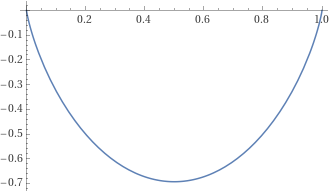
\includegraphics[width=0.9\linewidth]{Images/xlnx}
                \caption{$x$에 따른 $\Delta_\mathrm{mix}G$\footnote[1]{가로축은 $x$, 세로축은 $\Delta_\mathrm{mix}G/nRT$}}\label{f6a}
            \end{subfigure}
            \begin{subfigure}{0.5\textwidth}
                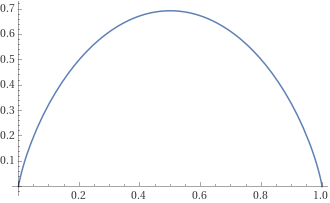
\includegraphics[width=0.9\linewidth]{Images/minusxlnx}
                \caption{$x$에 따른 $\Delta_\mathrm{mix}S$\footnote[2]{가로축은 $x$, 세로축은 $\Delta_\mathrm{mix}S/nR$}}\label{f6b}
            \end{subfigure}
        \end{figure}
        \par 실제 용액에서는 분자들 사이의 상호작용이 모두 다르다. 따라서 혼합 엔탈피가 0이 아닐 수 있고, 부피 변화 또한 0이 아닐 수 있다. 만약 
        혼합 엔트로피가 음수일 경우, 혼합의 Gibbs 에너지는 양수가 될 수 있다. 이 경우 액체의 혼합은 일어나지 않는다(Immiscible). 한편, 
        \textbf{부분적으로 섞이는(Partially miscible)} 경우도 있다. 이 경우 특정 비율까지만 혼합될 수 있다.
        \par 실제 용액과 이상 용액에서의 열역학 변수들의 차를 \textbf{초과 함수(Excess function, $X^E$)}라 한다. 이때 $X$는 열역학 변수를 의미한다. 
        초과 함수는 다음과 같이 정의된다:
        \begin{defn}[초과 함수]
        \begin{equation*}
            X^E = \Delta_\mathrm{mix}X-\Delta_\mathrm{mix}X^\mathrm{ideal}
        \end{equation*}
        \end{defn}
        예를 들어 초과 엔트로피 $S^E$를 생각할 수 있다. A와 B가 혼합될 때 초과 엔탈피 $H^E > 0$일 경우, 
        A-B 사이의 상호작용이 A-A와 B-B 사이의 상호작용보다 덜 선호된다는 것을 알 수 있다. 
        \par 이상 용액은 아니지만, 실제 용액의 좋은 모형으로 \textbf{정규 용액(Regular solution)}을 생각할 수 있다:
        \begin{defn}[정규 용액]
        정규 용액은 초과 엔탈피 $H^E \neq 0$이지만 
        초과 엔트로피 $S^E = 0$인 용액이다. 이는 두 종류의 분자가 무작위로 분포하나, 분자 간 상호작용의 크기는 같지 않은 경우로 생각할 수 있다.
        \end{defn}
        \par 정규 용액에서 초과 엔탈피는 다음과 같이 쓸 수 있다:
        \begin{obs}[정규 용액에서의 초과 엔탈피]\label{excessenth}
        \begin{equation*}
            H^E = n \xi RT x_A x_B
        \end{equation*}
        \end{obs}
        이때 $\xi$는 A-A 상호작용과 B-B 상호작용과 비교하여 A-B 상호작용의 에너지가 얼마나 되는지 나타내는 무차원 변수이다. 
        만약 $\xi<0$일 경우, A-B 상호작용이 더 선호되어 혼합은 발열 반응이 된다. 반대로 $\xi>0$일 경우, A-A와 B-B 상호작용이 더 선호되어 
        혼합은 흡열 반응이 된다. 이를 고려하여 정규 용액의 혼합 Gibbs 에너지를 구하면
        \begin{obs}[정규 용액의 혼합 Gibbs 에너지]\label{excessgibbs}
        \begin{equation*}
            \begin{aligned}
                \Delta_\mathrm{mix}G &= n\xi RT x_A x_B - T\left[-nR\left(x_A \ln{x_A}+x_B \ln{x_B}\right)\right]\\
                &= nRT\left(x_A \ln{x_A}+ x_B \ln{x_B} + \xi x_A x_B\right)
            \end{aligned}
        \end{equation*}
        \end{obs}
        과 같다. 이때 $\xi > 2$이면, $\Delta_\mathrm{mix}G$의 극소점이 두 개로 나뉜다. 이는 혼합물이 자발적으로 두 개의 상으로 나뉘는 것을 의미한다.
        \par 이제부터 용액의 총괄성(Colligative property)에 대해 살펴볼 것이다.
        \begin{defn}[총괄성]
        \textbf{총괄성(Colligative property)}이란, 용액의 물리적인 성질이 
        용질의 성질에 관계없이 용질 입자의 개수에 의존하는 것을 의미한다. 증기 압력 내림, 끓는점 오름, 어는점 내림, 삼투압이 총괄성의 예시이다.
        \end{defn}
        총괄성을 보이기 위해서는 두 가지 가정이 필요하다:
        \begin{enum}
            \item 용질은 비휘발성이다. 즉 용질은 증기 압력에 관여하지 않는다.
            \item 용질은 고체 용매에 녹지 않는다. 즉 용매가 응고하면 순수한 고체 물질이 된다. 
        \end{enum}
        총괄성은 액체 용매에 용질이 녹을 때 액체의 화학 퍼텐셜이 감소하는 것으로부터 출발한다. 이상 용액에서(즉 Raoult 법칙을 만족하면), 순수한 액체 용매의 
        화학 퍼텐셜 $\mu_A^\ast$에서 용질이 녹으면 화학 퍼텐셜은 $-RT\ln{x_A}$만큼 감소한다. 즉 $\mu_A = \mu_A^\ast + RT \ln{x_A}$가 된다. 2번째 가정에 의해, 
        용매 증기나 고체 용매는 화학 퍼텐셜에 영향을 미치지 않는다. 따라서 Figure \ref{f7}과 같이, 어는점 내림(Freezing point depression)과 
        끓는점 오름(Boiling point elevation)이 나타난다.
        \begin{figure}[H]
            \centering
            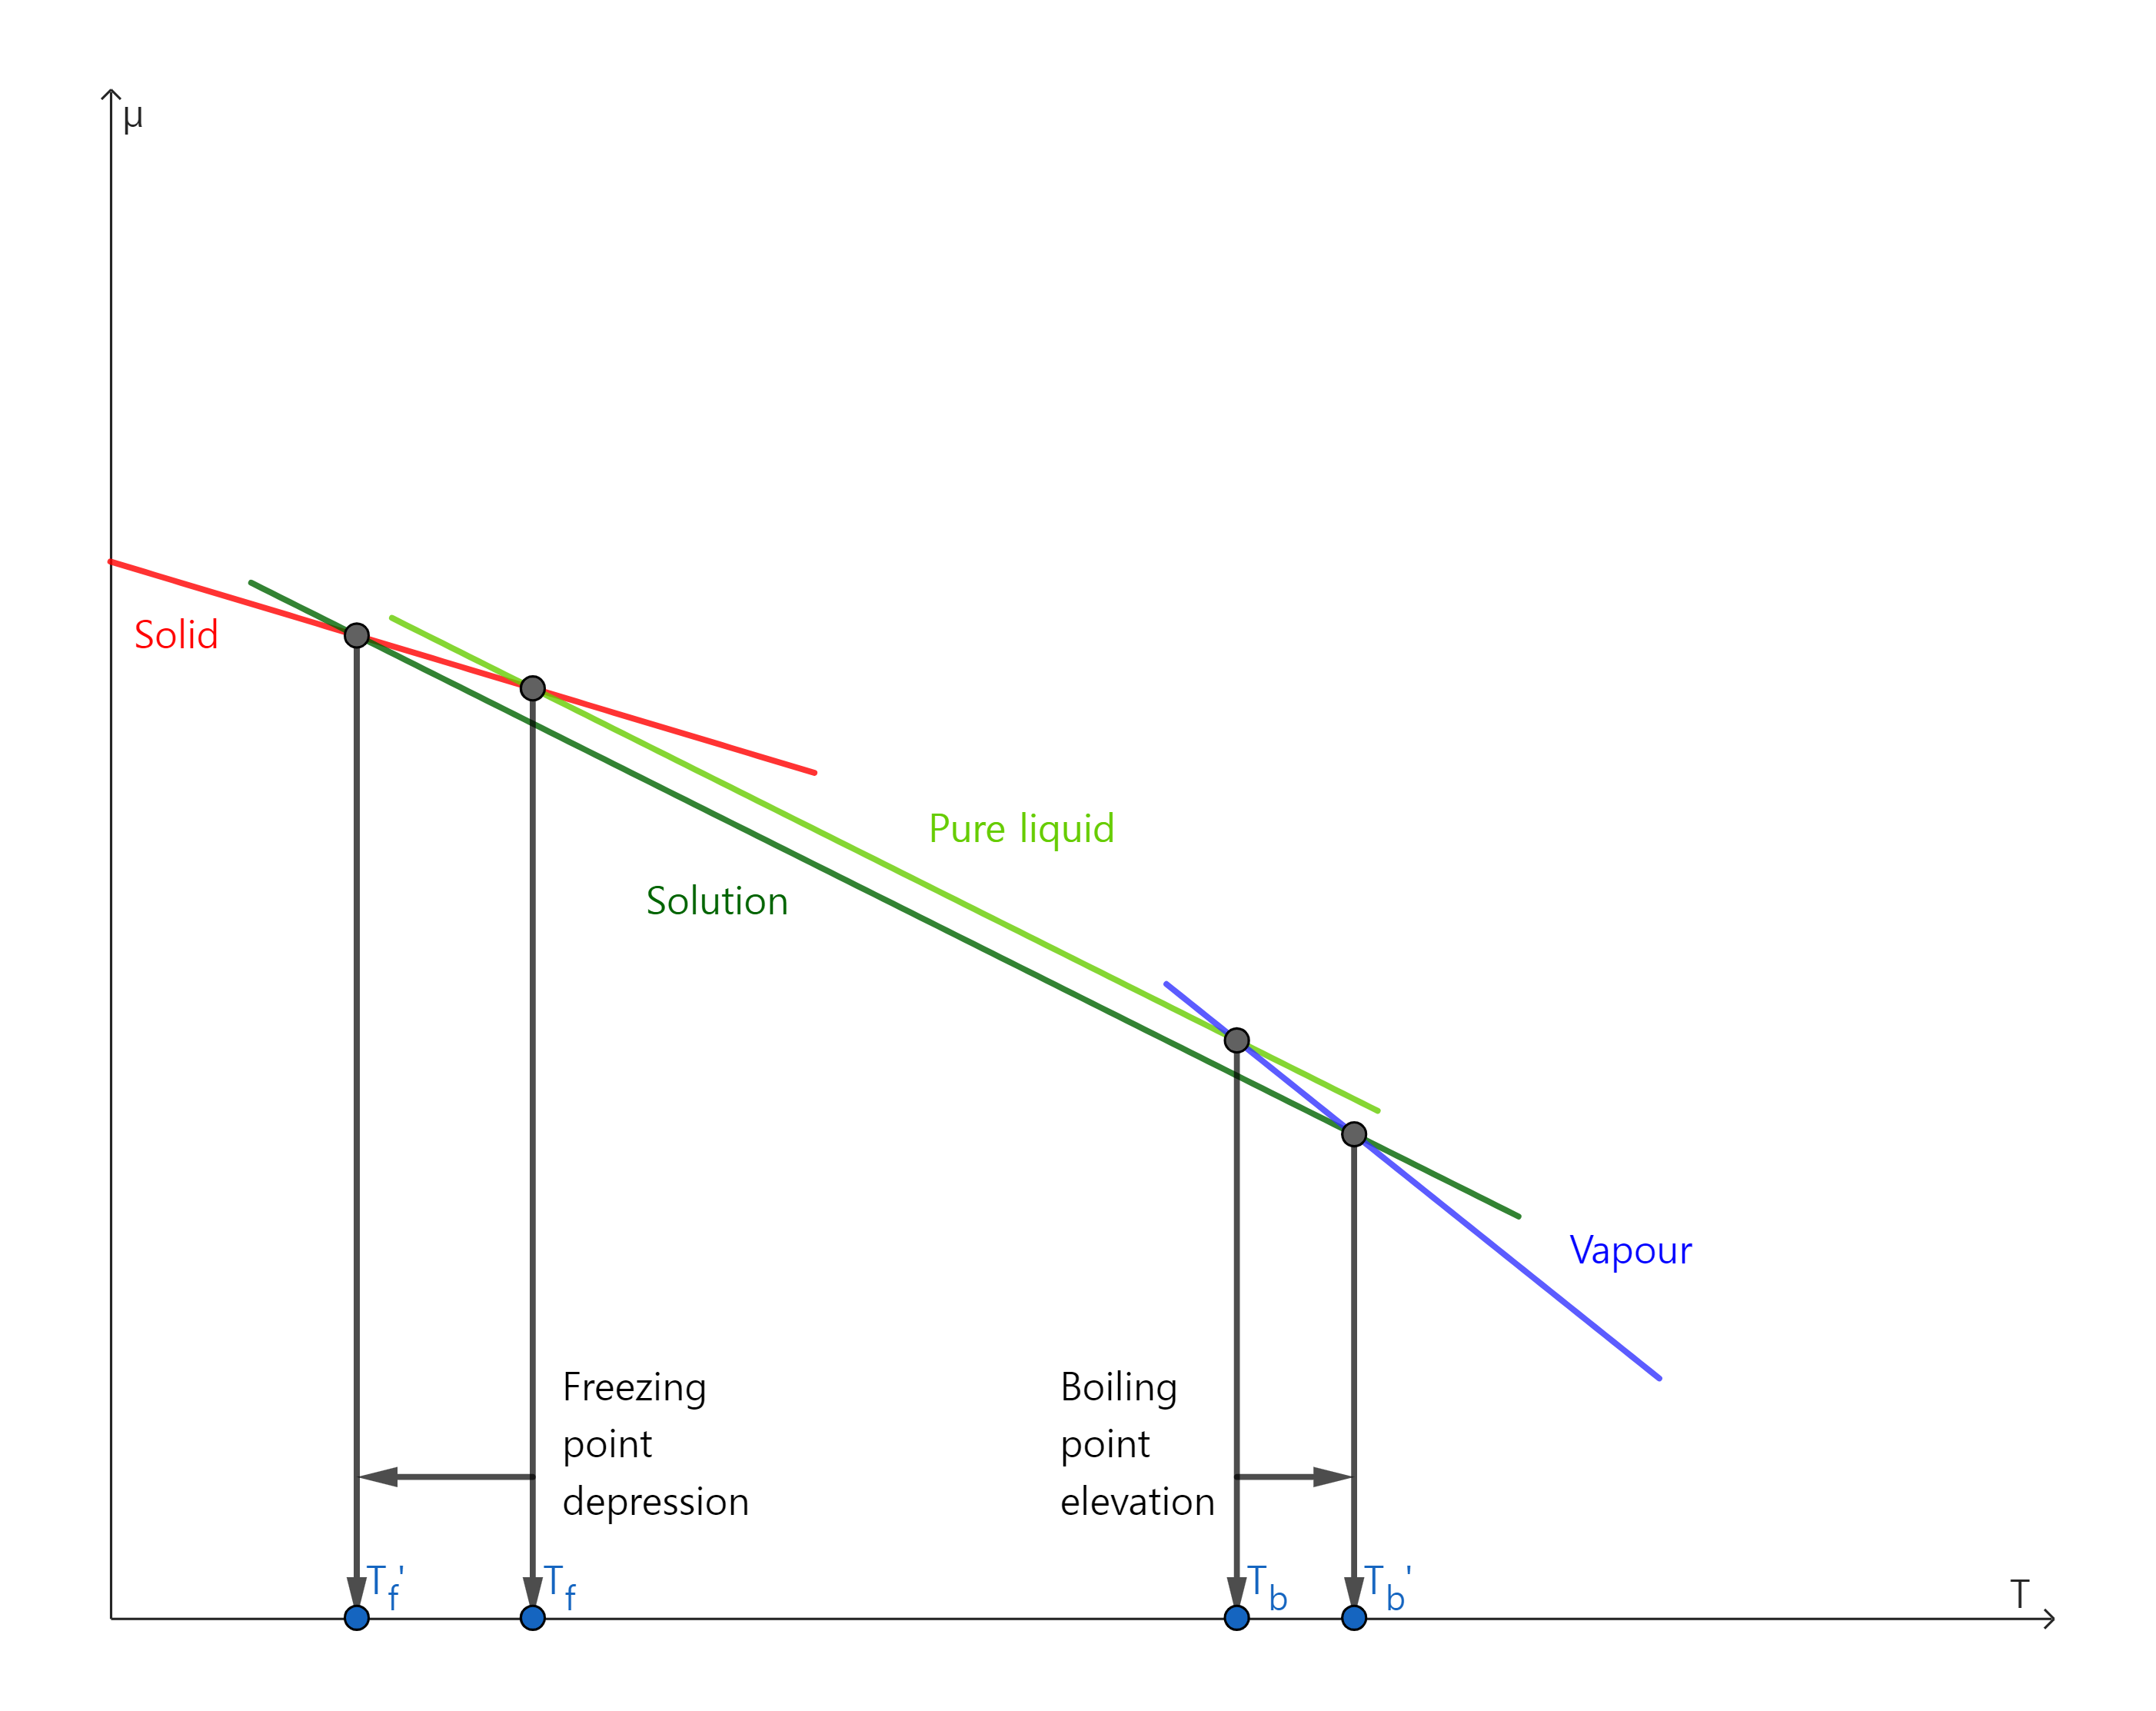
\includegraphics[scale=0.4]{Images/chempotcoll}
            \caption{상태 변화의 화학 퍼텐셜 변화}\label{f7}
        \end{figure}
        이는 이상 용액에서도 나타나는 현상이다. 따라서 이러한 현상은 엔트로피에 의한 것이다.
        \par 먼저 끓는점 오름을 유도해 보자.
        \begin{proof}[끓는점 오름]
        $\mu_A^\ast\left(\mathrm{g}\right)=\mu_A^\ast\left(\mathrm{l}\right)+RT\ln{x_A}$로부터 시작한다. 이때 
        별표는 순수한 물질에서의 상태를 나타낸다. 다시 정리하면 다음을 만족한다:
        $$
        \ln{x_A}=\frac{\mu_A^\ast\left(\mathrm{g}\right)-\mu_A^\ast\left(\mathrm{l}\right)}{RT}=\frac{\Delta_\mathrm{vap}G}{RT}
        $$
        이때 Gibbs-Helmholtz 방정식 (\ref{gheqn})을 이용해, 양변을 T로 미분하면
        $$
        \frac{\difform \ln{x_A}}{\difform T}=\frac{1}{R} \frac{\difform \left(\Delta_\mathrm{vap}G/T\right)}{\difform T}=-\frac{\Delta_\mathrm{vap}H}{RT^2}
        $$
        이 성립한다. 따라서 $\displaystyle\difform \ln{x_A}=-\frac{\Delta_\mathrm{vap}H}{RT^2}\difform T$에서, 
        양변을 적분하면 
        $$
        \int_{0}^{\ln{x_A}}\difform \ln{x_A^\prime}=-\frac{1}{R}\int_{T^\ast}{T}\frac{\Delta_\mathrm{vap}H}{T^{\prime 2}}\difform T^\prime
        $$
        이 성립한다. 이를 A와 B가 혼합된 이원계 혼합물에서 계산하면 다음과 같다:
        $$
        \ln{\left(1-x_B\right)}=\frac{\Delta_\mathrm{vap}H}{R}\left(\frac{1}{T}-\frac{1}{T^\ast}\right)
        $$
        $t <\!< 1$일 때 $\ln{\left(1-t\right)}\approx -t$로 근사할 수 있고, $T\approx T^\ast$에서 $\displaystyle\frac{1}{T^\ast}-\frac{1}{T}\approx \frac{T-T^\ast}{{T^\ast}^2} = \frac{\Delta T_b}{{T^\ast}^2}$이므로 
        다음이 성립한다:
        \begin{equation*}
            x_B = \frac{\Delta_\mathrm{vap}H}{R}\times\frac{\Delta T_b}{{T^\ast}^2}
        \end{equation*}
        이때 $K = \frac{R{T^\ast}^2}{\Delta_\mathrm{vap}H}$로 정의하면,
        \begin{equation*}
            \Delta T_b = K x_B
        \end{equation*}
        가 성립한다. 이를 \textbf{끓는점 오름(Elevation of boiling point)}이라 한다.
        \end{proof}
        \par 실제로는 경험적으로 몰랄 농도 $b$를 이용하여
        \begin{equation*}
            \Delta T_b = K_b b
        \end{equation*}
        를 쓴다. 이 $K_b$를 \textbf{끓는점 오름 상수(Boiling-point constant)}라 한다.
        \begin{proof}[어는점 내림]
        어는점 내림도 마찬가지로
        $$
        \mu_A^\ast\left(\mathrm{s}\right)=\mu_A^\ast\left(\mathrm{l}\right)+RT\ln{x_A}
        $$
        에서 출발하여 다음과 같은 식을 얻을 수 있다:
        \begin{equation*}
            \Delta T_f = K^\prime x_B
        \end{equation*}
        이때 $\displaystyle K^\prime = \frac{R{T^\ast}^2}{\Delta_\mathrm{fus}H}$이고, 이를 \textbf{어는점 내림(Freezing point depression)}이라 한다.
        \end{proof}
        \par 실제로는 경험적으로 몰랄 농도 $b$를 이용하여 
        \begin{equation*}
            \Delta T_f = K_f b
        \end{equation*}
        를 쓴다. 이 $K_f$를 \textbf{어는점 내림 상수(Freezing-point constant)}라 한다.
        \par 용해도의 경우에는 총괄성에 해당되지는 않지만(용질의 성질에 영향을 받으므로), 이상 용액은 열역학적으로 다음 식을 만족한다:
        \begin{equation*}
            \ln{x_B}=\frac{\Delta_\mathrm{fus}H}{R}\left(\frac{1}{T_f}-\frac{1}{T}\right)
        \end{equation*}
        \begin{defn}[삼투 현상과 삼투압]
        \textbf{삼투 현상(Osmosis)}은 서로 농도가 다른 두 용액이, 용매 분자는 통과시키지만 용질은 통과시키지 않는 \textbf{반투막(Semipermeable membrane)}을 사이에 
        두고 분리되어 있을 때 저농도에서 고농도로 용매가 흐르는 현상이다. \textbf{삼투압(Osmotic pressure, $\Pi$)}은 이때 용매의 흐름을 막기 위해 고농도 용액에 
        가해야 하는 압력이다.
        \end{defn}
        삼투 현상을 이용하여 거대 분자의 분자량을 측정할 수 있다. 이를 \textbf{삼투법(Osmometry)}이라 한다. 삼투 현상 또한 총괄성에 속한다. 
        \begin{proof}[삼투 현상]
        먼저 순수한 용매와 용액이 반투막으로 분리되어 있다고 하자. 평형 상태에서 다음 등식으로부터 출발한다:
        $$
        \mu_A^\ast\left(p\right)=\mu_A\left(x_A,p+\Pi\right)
        $$
        이때 $\mu_A\left(x_A,p+\Pi\right)=\mu_A^\ast\left(p+\Pi\right)+RT\ln{x_A}$를 만족하고, 이를 대입하면 다음이 성립한다:
        $$
        \mu_A^\ast\left(p+\Pi\right)=\mu_A^\ast\left(p\right)-RT\ln{x_A}
        $$
        식 \ref{gibbspartial}에 의해 $G_m\left(p_f\right)=G_m\left(p_i\right)+\int_{p_i}^{p_f}V_m \difform p$를 만족하므로, 다음을 
        만족한다:
        $$
        \mu_A^\ast \left(p+\Pi\right)=\mu_A^\ast\left(p\right) + \int_{p}^{p+\Pi}V_m \difform p
        $$
        위 식에서 $-RT \ln{x_A}=\int_{p}^{p+\Pi}V_m \difform p$을 만족하고, 용매의 몰 부피가 거의 일정하다고 가정하면 
        $\int_{p}^{p+\Pi}V_m\difform p = V_m \Pi$를 만족한다. 따라서
        $$
        -RT\ln{x_A}=V_m\Pi
        $$
        를 만족한다. 이때 $-RT\ln{x_A} = -RT\ln{\left(1-x_B\right)} \approx RTx_B$를 만족하므로, 묽은 용액의 삼투압은 다음과 같다:
        \begin{equation*}
            RTx_B=\Pi V_m
        \end{equation*}
        만약 B의 농도가 매우 묽을 경우, $x_B \approx n_B/n_A$로 근사할 수 있다. 따라서 $RT n_B \approx n_A \Pi V_m$을 만족하고, 
        $n_A V_m \approx V$이기 때문에 $RT n_B = \Pi V$, 즉 $V$를 양변에 나누면 다음과 같은 \textbf{van 't Hoff 방정식(van 't Hoff equation)}을 
        만족한다:
        \begin{equation*}
            \Pi = \left[ B \right]RT
        \end{equation*}
        이때 $\left[ J \right]$는 $J$의 몰 농도를 의미한다.
        \end{proof}
        여기서도 마찬가지로 비리얼 급수를 구할 수 있다 \textbf{(삼투 비리얼 급수(Osmotic virial expansion))}:
        $$
        \Pi = \left[ J\right]RT \left\{ 1+B\left[J\right]+\cdots\right\}
        $$
        이때 경험적인 계수 $B$는 \textbf{삼투 비리얼 계수(Osmotic virial coefficient)}라 한다.
    \section{이원계 상평형도: 액체}\label{ch5sub3}
        \hspace{\parindent}\textbf{증기 압력 그림(Vapour pressure diagram)}에서는 주어진 압력에서 평형을 이루는 분율을 나타낸 상평형도이다.
        두 휘발성 액체의 이상 용액에서, 부분 증기 압력은 Raoult 법칙에 의해 몰 분율과 비례한다:
        \begin{equation*}
            p_J = x_J p_J^\ast
        \end{equation*}
        따라서 혼합물의 총 증기 압력은 다음 Figure \ref{f8}을 따른다:\\
        \begin{figure}[H]
            \centering
            \begin{tikzpicture}
                \draw[black, thick, ->] (-3,-2.5) -- (-3,2.5) node[rotate = 90, midway, above] {압력, $p$};
                \draw[black, thick] (-3,-2.5) -- (3,-2.5) node[midway, below] {A의 몰 분율, $x_A$};
                \draw[black, thick, ->] (3,-2.5) -- (3,2.5);
                \draw[black, thick] (-3,-1.25) -- (3,1.5);
                \draw[black, thick, ->] (-2,-1.25) -- (-3,-1.25) node[midway, right=12pt] {$p_B^\ast$};
                \draw[black, thick, ->] (2,1.5) -- (3,1.5) node[midway, left=12pt] {$p_A^\ast$};
                \node at (-1,1.5) {Liquid};
                \node at (1,-1.5) {Vapour};
                \node[node font=\small, rotate=90, below right] at (-3,-2.5) {Pure B};
                \node[node font=\small, rotate=90, above right] at (3,-2.5) {Pure A};
                \node[below] at (-3,-2.5) {0};
                \node[below] at (3,-2.5) {1};
            \end{tikzpicture}
            \caption{Raoult 법칙을 만족할 때의 총 증기 압력}\label{f8}
        \end{figure}
        따라서 $p = p_A + p_B$를 따른다. 만약 증기에서의 몰 분율과 액체에서의 몰 분율이 다를 경우, 
        증기의 몰 분율 $y_J$를 다음과 같이 정의한다:
        \begin{equation*}
            y_J = \frac{p_J}{p}
        \end{equation*}
        만약 이상 용액일 경우, 액체의 몰 분율 $x_J$에 대해 다음을 만족한다:
        \begin{equation*}
            y_A = \frac{x_A p_A^\ast}{p_B^\ast + \left(p_A^\ast - p_B^\ast\right)x_A}
        \end{equation*}
        또한 $y_B = 1-y_A$를 만족한다. $p_A^\ast$와 $p_B^\ast$는 각 분자의 휘발성과 관련이 있고, 이 둘의 비율로 증기에 
        무엇이 더 많을지 예측할 수 있다. 즉 $p_A^\ast / p_B^\ast > 1$일 때, $y_A > x_A$를 만족한다.
        \par \textbf{온도-분율 그림(Temperature-composition diagram)}은 주어진 온도에서 평형 상태를 이루는 분율을 나타낸 상평형도이다. 
        이때, 압력은 주로 1 atm에서 측정한다. 이때 액체 상이 아래에 위치하고, 액체 상의 경계는 그 분율에서의 끓는점을 나타낸다. 또한 
        기체 상의 경계는 특정 온도에서 기체의 분율을 나타낸다. 그림은 다음 Figure \ref{f9}와 같다:\\
        \begin{figure}[H]
            \centering
            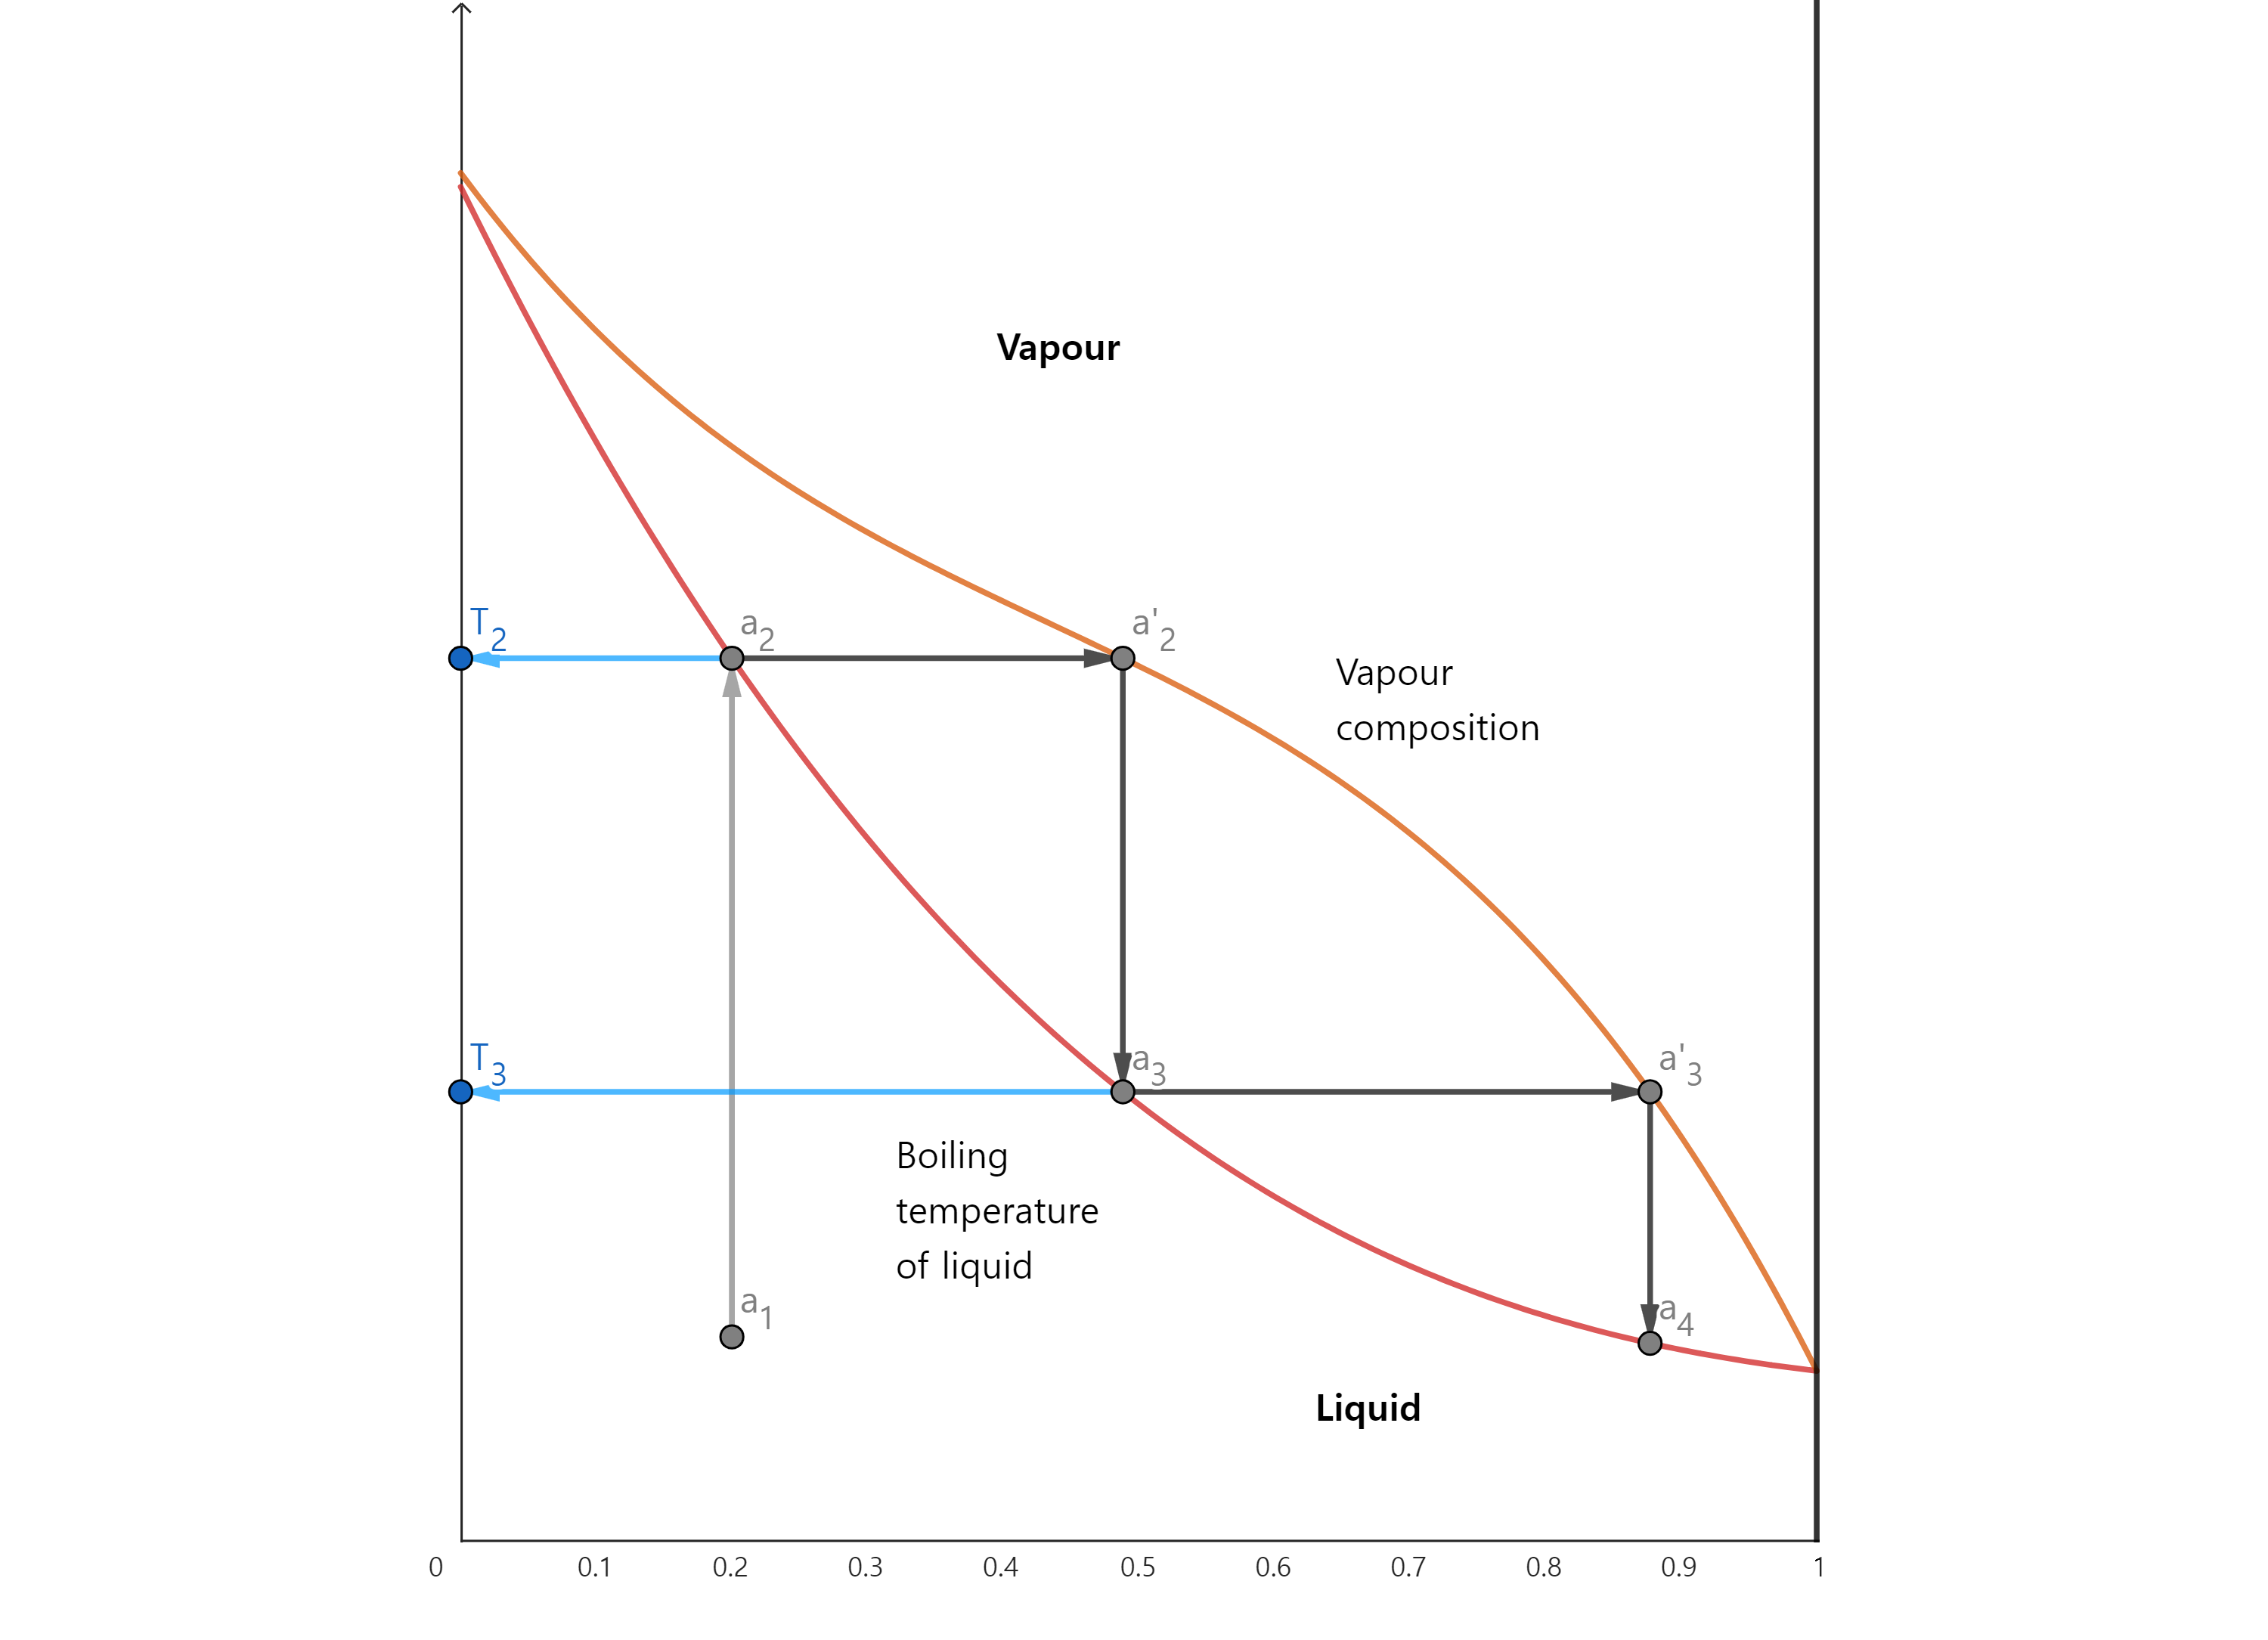
\includegraphics[scale=8]{Images/lgphasediag}
            \caption{온도-분율 그림}\label{f9}
        \end{figure}
        이는 증류 과정에서 중요하다. 즉, 같은 온도에서 기체를 응축하면 응축된 액체의 구성 분율은 달라진다. 이러한 그림에서 
        상 경계는 \textbf{공존 곡선(Coexistence curve)}이라고도 한다.
        \par 이제부터 지레 규칙에 대해 알아볼 것이다. 다음과 같은 Figure \ref{f10}을 생각하자:
        \begin{figure}[H]
            \centering
            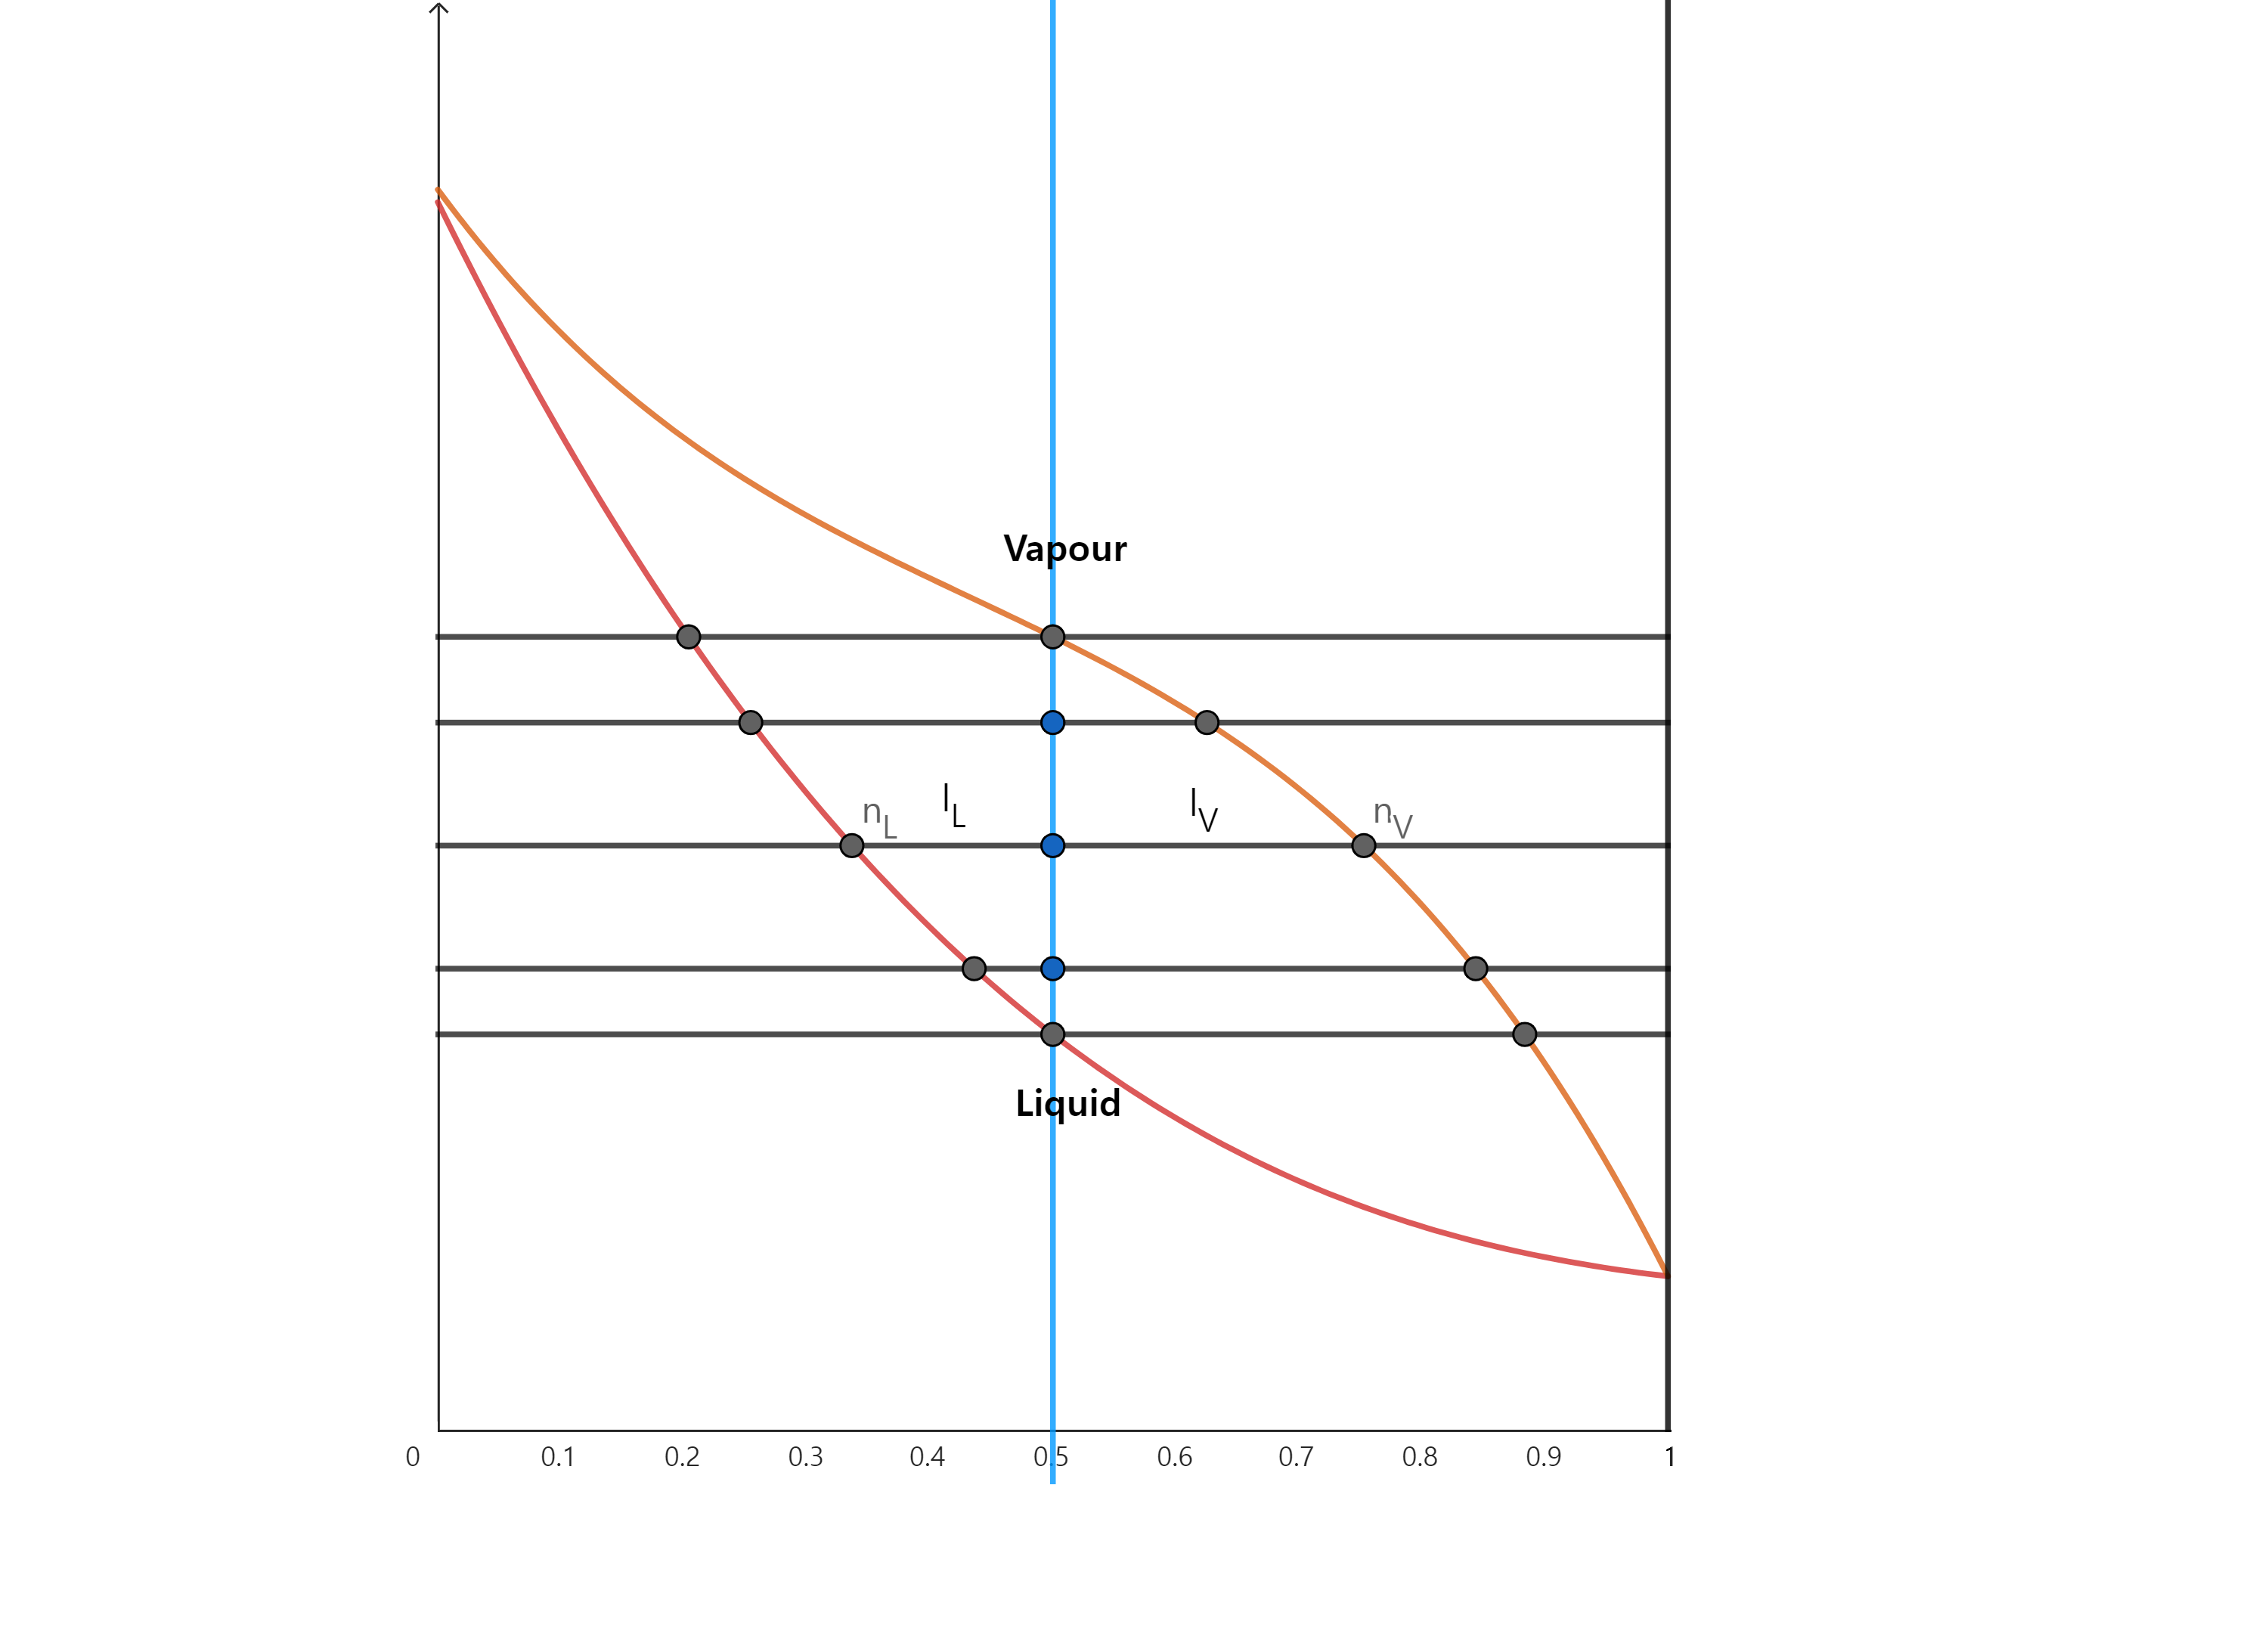
\includegraphics[scale=7]{Images/lgphasediaglever}
            \caption{온도-분율 그림에서의 지레 규칙}\label{f10}
        \end{figure}
        이때 구하고자 하는 몰 분율을 $z_A$라 하자. 이 온도에서 기체상은 $x_A$, 액체상은 $y_A$의 몰 분율을 가지고 있다고 하자. 이때 다음을 만족한다:
        \begin{equation*}
            n_A = n_L x_A + n_V y_A
        \end{equation*}
        또한 $z_A$에서 
        \begin{equation*}
            n_A = nz_A = n_L z_A + n_V z_A
        \end{equation*}
        를 만족한다. 이 둘을 연립하면 
        \begin{equation*}
            n_L\left(z_A - x_A\right) = n_V \left(y_A - z_A\right)
        \end{equation*}
        이때 주어진 점에서 각 공존 곡선까지의 '거리'를 다음과 같이 정의하자:
        \begin{align*}
        l_L &= z_A-x_A\\
        l_V &= y_A-z_A
        \end{align*}
        따라서 다음과 같은 \textbf{지레 규칙(Lever rule)}을 유도할 수 있다:
        \begin{law}[지레 규칙]
        \begin{equation*}
            n_L l_L = n_V l_V
        \end{equation*}
        \end{law}
        이러한 지레 규칙은 액체-기체 상평형도뿐만 아니라 모든 상평형도에서 성립한다. 또한, 일정한 몰 분율을 나타낸 직선을 \textbf{등치선(Isopleth)}이라 한다.
        \par \textbf{단순 증류(Simple distillation)}는 기화된 기체를 응축하여 분리하는 방법이다. 이는 비휘발성 고체나 용질로부터 휘발성 액체를 분리하는 데 이용한다. 
        또한 \textbf{분별 증류(Fractional distillation)}는 이러한 증류를 여러 번 하는 방법이다. 이때 분별 증류관의 효율은 
        \textbf{이론단수(Theoretical plates)}\footnote[13]{이 개념은 분석화학에서 크로마토그래피를 다룰 때에도 사용한다.}를 통해 나타낸다.
        \par 물과 에탄올의 혼합물과 같이, 증류 시 일정 지점을 기준으로 넘어갈 수 없는 경우가 존재한다. 이러한 경우를 \textbf{공비혼합물(Azeotrope)}이라 한다. 
        A-B 혼합물이 공비혼합물을 이룰 때, A-B 분자 간 상호작용이 액체를 안정화할 경우 초과 Gibbs 에너지 $G^E <0$을 만족한다. 따라서 증류 시 
        남아 있는 액체 혼합물의 분율이 일정 지점을 넘어갈 수 없다(High-boiling azeotrope). 또한, A-B 분자 간 상호작용이 액체를 불안정화할 경우, 
        초과 Gibbs 에너지 $G^E >0$을 만족한다. 따라서 증류 시 증기의 분율이 일정 지점을 넘어갈 수 없다(Low-boiling azeotrope). 다음 Figure \ref{f11}은 물-에탄올 혼합물의 
        온도-분율 그림이다\footnote[14]{https://www.science.smith.edu/~jbrady/petrology/igrocks-diagrams/binary/H2O-ethanol.php}:\\
        \begin{figure}[H]
            \centering
            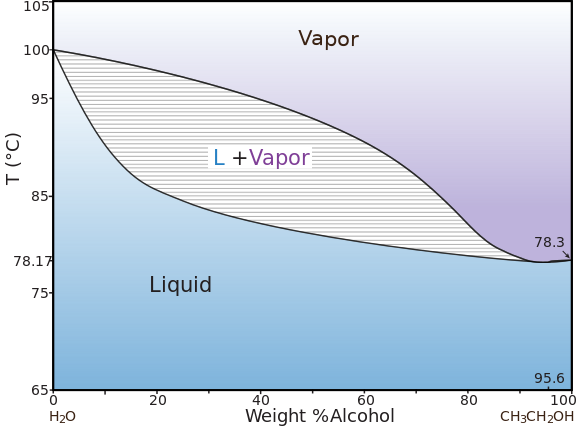
\includegraphics[scale=0.5]{Images/waterethanolazeo}
            \caption{물-에탄올 혼합물의 온도-분율 그림}\label{f11}
        \end{figure}
        이때 공비점인 에탄올 95.6 wt\%에서는 액체의 몰 분율과 기체의 몰 분율이 같아 더 이상 증류할 수 없다.
        \par 이제 섞이지 않는 두 액체에 대해 살펴보자. 서로 매우 적게 녹아있기 때문에, 총 증기 압력은 $p=p_A^\ast + p_B^\ast$에 가깝다. 
        만약 대기압과 총 증기 압력이 같아지면, 용액은 끓기 시작하고 용액에서 용해된 물질들이 분리되어 나온다. 
        대기압과 총 증기 압력이 같아지면 용액이 끓기 시작하는 성질을 이용한 증류를 \textbf{증기 증류(Steam distillation)}라고 한다. 
        이를 이용하면 열에 민감하고 물에 녹지 않는 유기물들을 끓는점보다 낮은 온도에서 분리할 수 있다. 만약 유기물의 휘발성이 낮다면, 
        증류가 어려울 수 있다.
        \par 액체-액체 상평형도는 \textbf{부분적으로 섞이는(Partially miscible)} 액체에 대해 적용할 수 있다. 일정 온도에서 일정 비율의 
        부분적으로 섞이는 액체 둘을 혼합하면 두 상으로 나뉜다. 즉 다음 Figure \ref{f12}와 같다:\\
        \begin{figure}[H]
            \centering
            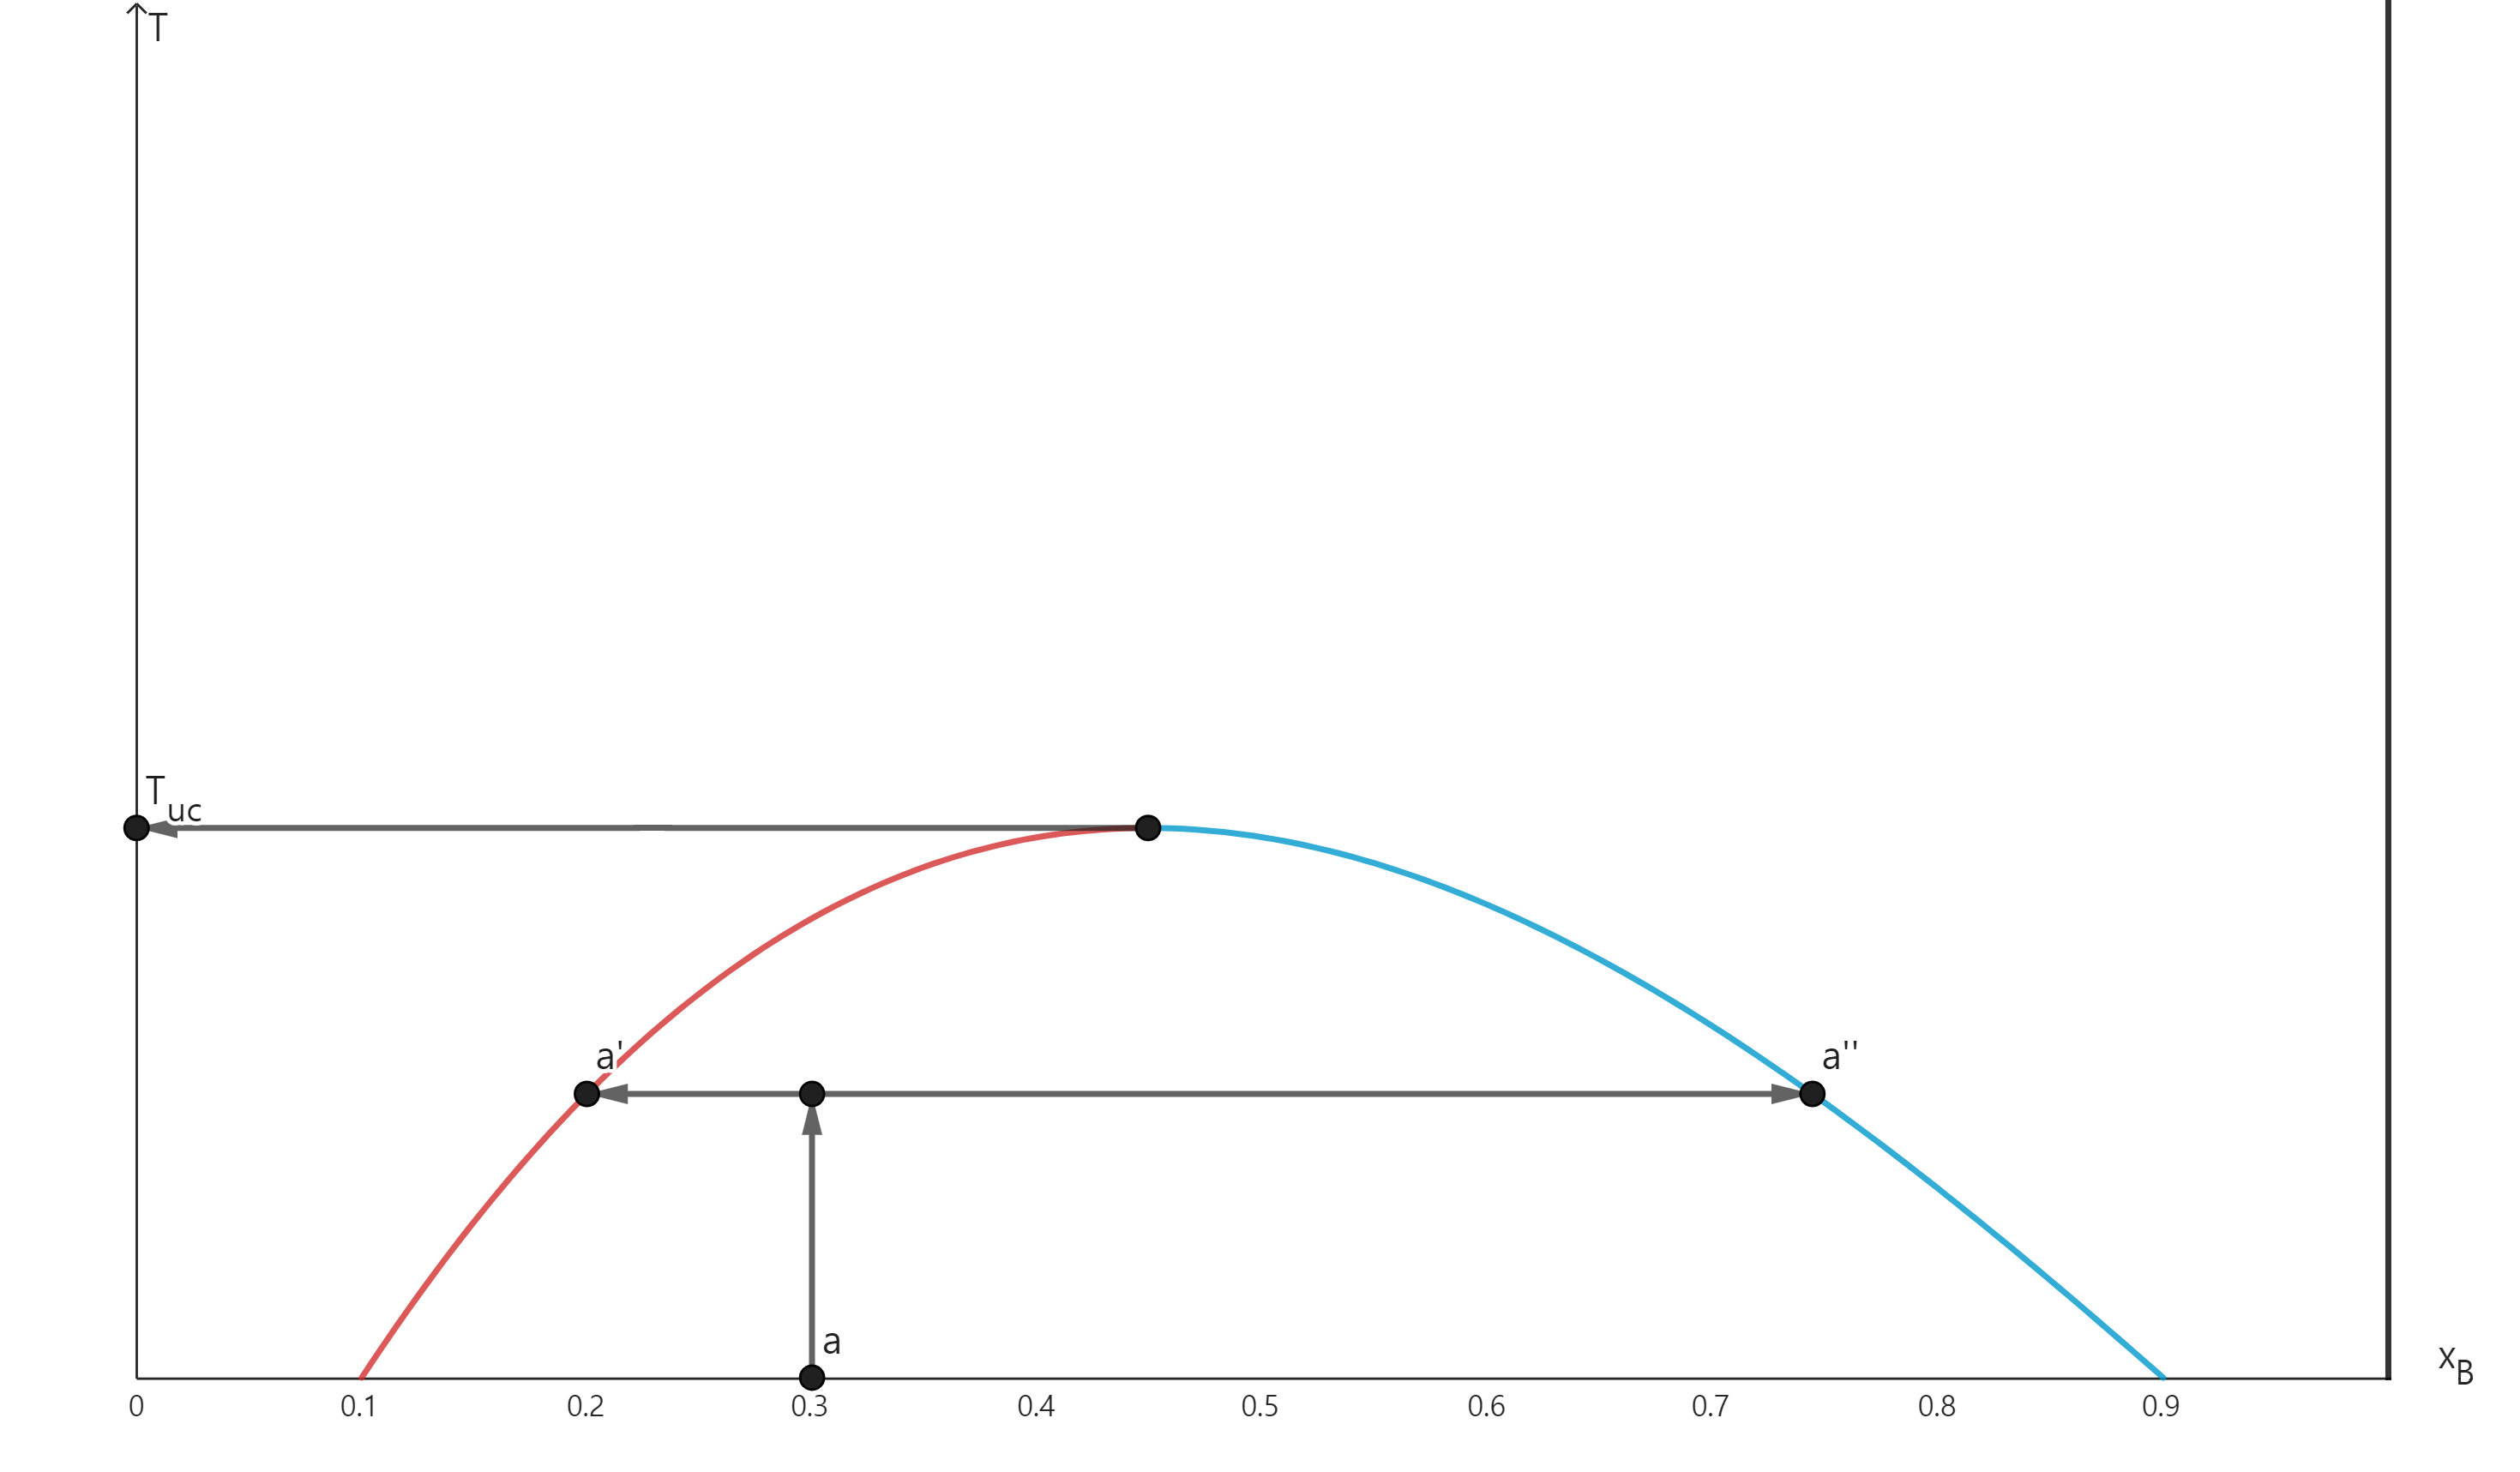
\includegraphics[scale=12]{Images/lldiaguc}
            \caption{액체-액체 상평형도}\label{f12}
        \end{figure}
        그림에서 나뉘는 부분은 $P=2$이고, 나뉘지 않는 부분은 $P=1$이다.
        \par 그림에서, $T_{uc}$ 이상의 온도에서는 어떤 분율을 취하더라도 완전히 섞인다. 이 온도를 
        \textbf{상부 임계 용해 온도(Upper critical solution temperature, UCST)}라 한다. 이 온도 이상에서는 분리되는 경우보다 
        섞이는 경우가 열역학적으로 유리하기 때문이다. 이를 열역학적으로 해석하자. 
        \par 식 \ref{excessenth}에서 도입한 $\xi$를 이용하자. $H^E = n\xi RTx_A x_B$이다. $\xi>2$일 때, 혼합 Gibbs 에너지는 극소점이 
        두 개 생긴다. 따라서 $\xi>2$일 때 상 분리가 발생한다. 이 최소점은 $\partial \Delta_\mathrm{mix}G/\partial x_A = 0$을 풀면 
        구할 수 있다. \ref{excessgibbs}로부터,
        \begin{equation*}
            \begin{aligned}
                &\left(\frac{\partial \Delta_\mathrm{mix}G}{\partial x_A}\right)_{T,p} \\
                &= nRT\left(\frac{\partial\left\{x_A\ln{x_A}+\left(1-x_A\right)\ln{\left(1-x_A\right)}+\xi x_A\left(1-x_A\right)\right\}}{\partial x_A}\right)_{T,p}\\
                &= nRT\left\{\ln{x_A}+1-\ln{\left(1-x_A\right)}-1+\xi\left(1-2x_A\right)\right\}\\
                &= nRT\left\{\ln{\frac{x_A}{1-x_A}}+\xi\left(1-2x_A\right)\right\}
            \end{aligned}
        \end{equation*}
        이므로 다음 방정식을 풀면 최소점을 구할 수 있다:
        \begin{equation*}
            \ln{\frac{x_A}{1-x_A}}=-\xi\left(1-2x_A\right)
        \end{equation*}
        이때 이 방정식은 해석적으로 풀 수 없으므로, 수치적으로 풀 경우 $\xi > 2$에서 상이 분리되는 것을 알 수 있다.
        \par 몇몇 계에서는 \textbf{하부 임계 용해 온도(Lower critical solution temperature, LCST; $T_{lc}$)}를 가진다. 
        이 경우 일정 온도 이하에서는 상이 분리되지 않으나, $T_\mathrm{lc}$ 이상에서는 상이 분리된다. 이는 저온에서 
        약한 복합체(complex)를 이루나, 그 이상의 온도에서 이러한 복합체가 분해되기 때문이다. 
        때에 따라 UCST와 LCST를 모두 가질 수 있다. 이는 낮은 온도에서는 약한 복합체를 이루고, LCST와 UCST 사이에서는 복합체가 분해된다. 
        이후 UCST 이상에서는 분자의 열운동이 혼합물의 상을 하나로 만든다. 이러한 혼합물의 예시는 니코틴과 물의 혼합물이 있다.
        \par 이러한 부분적으로 섞이는 용액을 증류할 때에도 상평형도를 이용할 수 있다. 
    \section{이원계 상평형도: 고체}
        \hspace{\parindent} 다음 Figure \ref{f13}과 같은 고체-액체 상평형도를 생각하자:\\
        \begin{figure}[H]
            \centering
            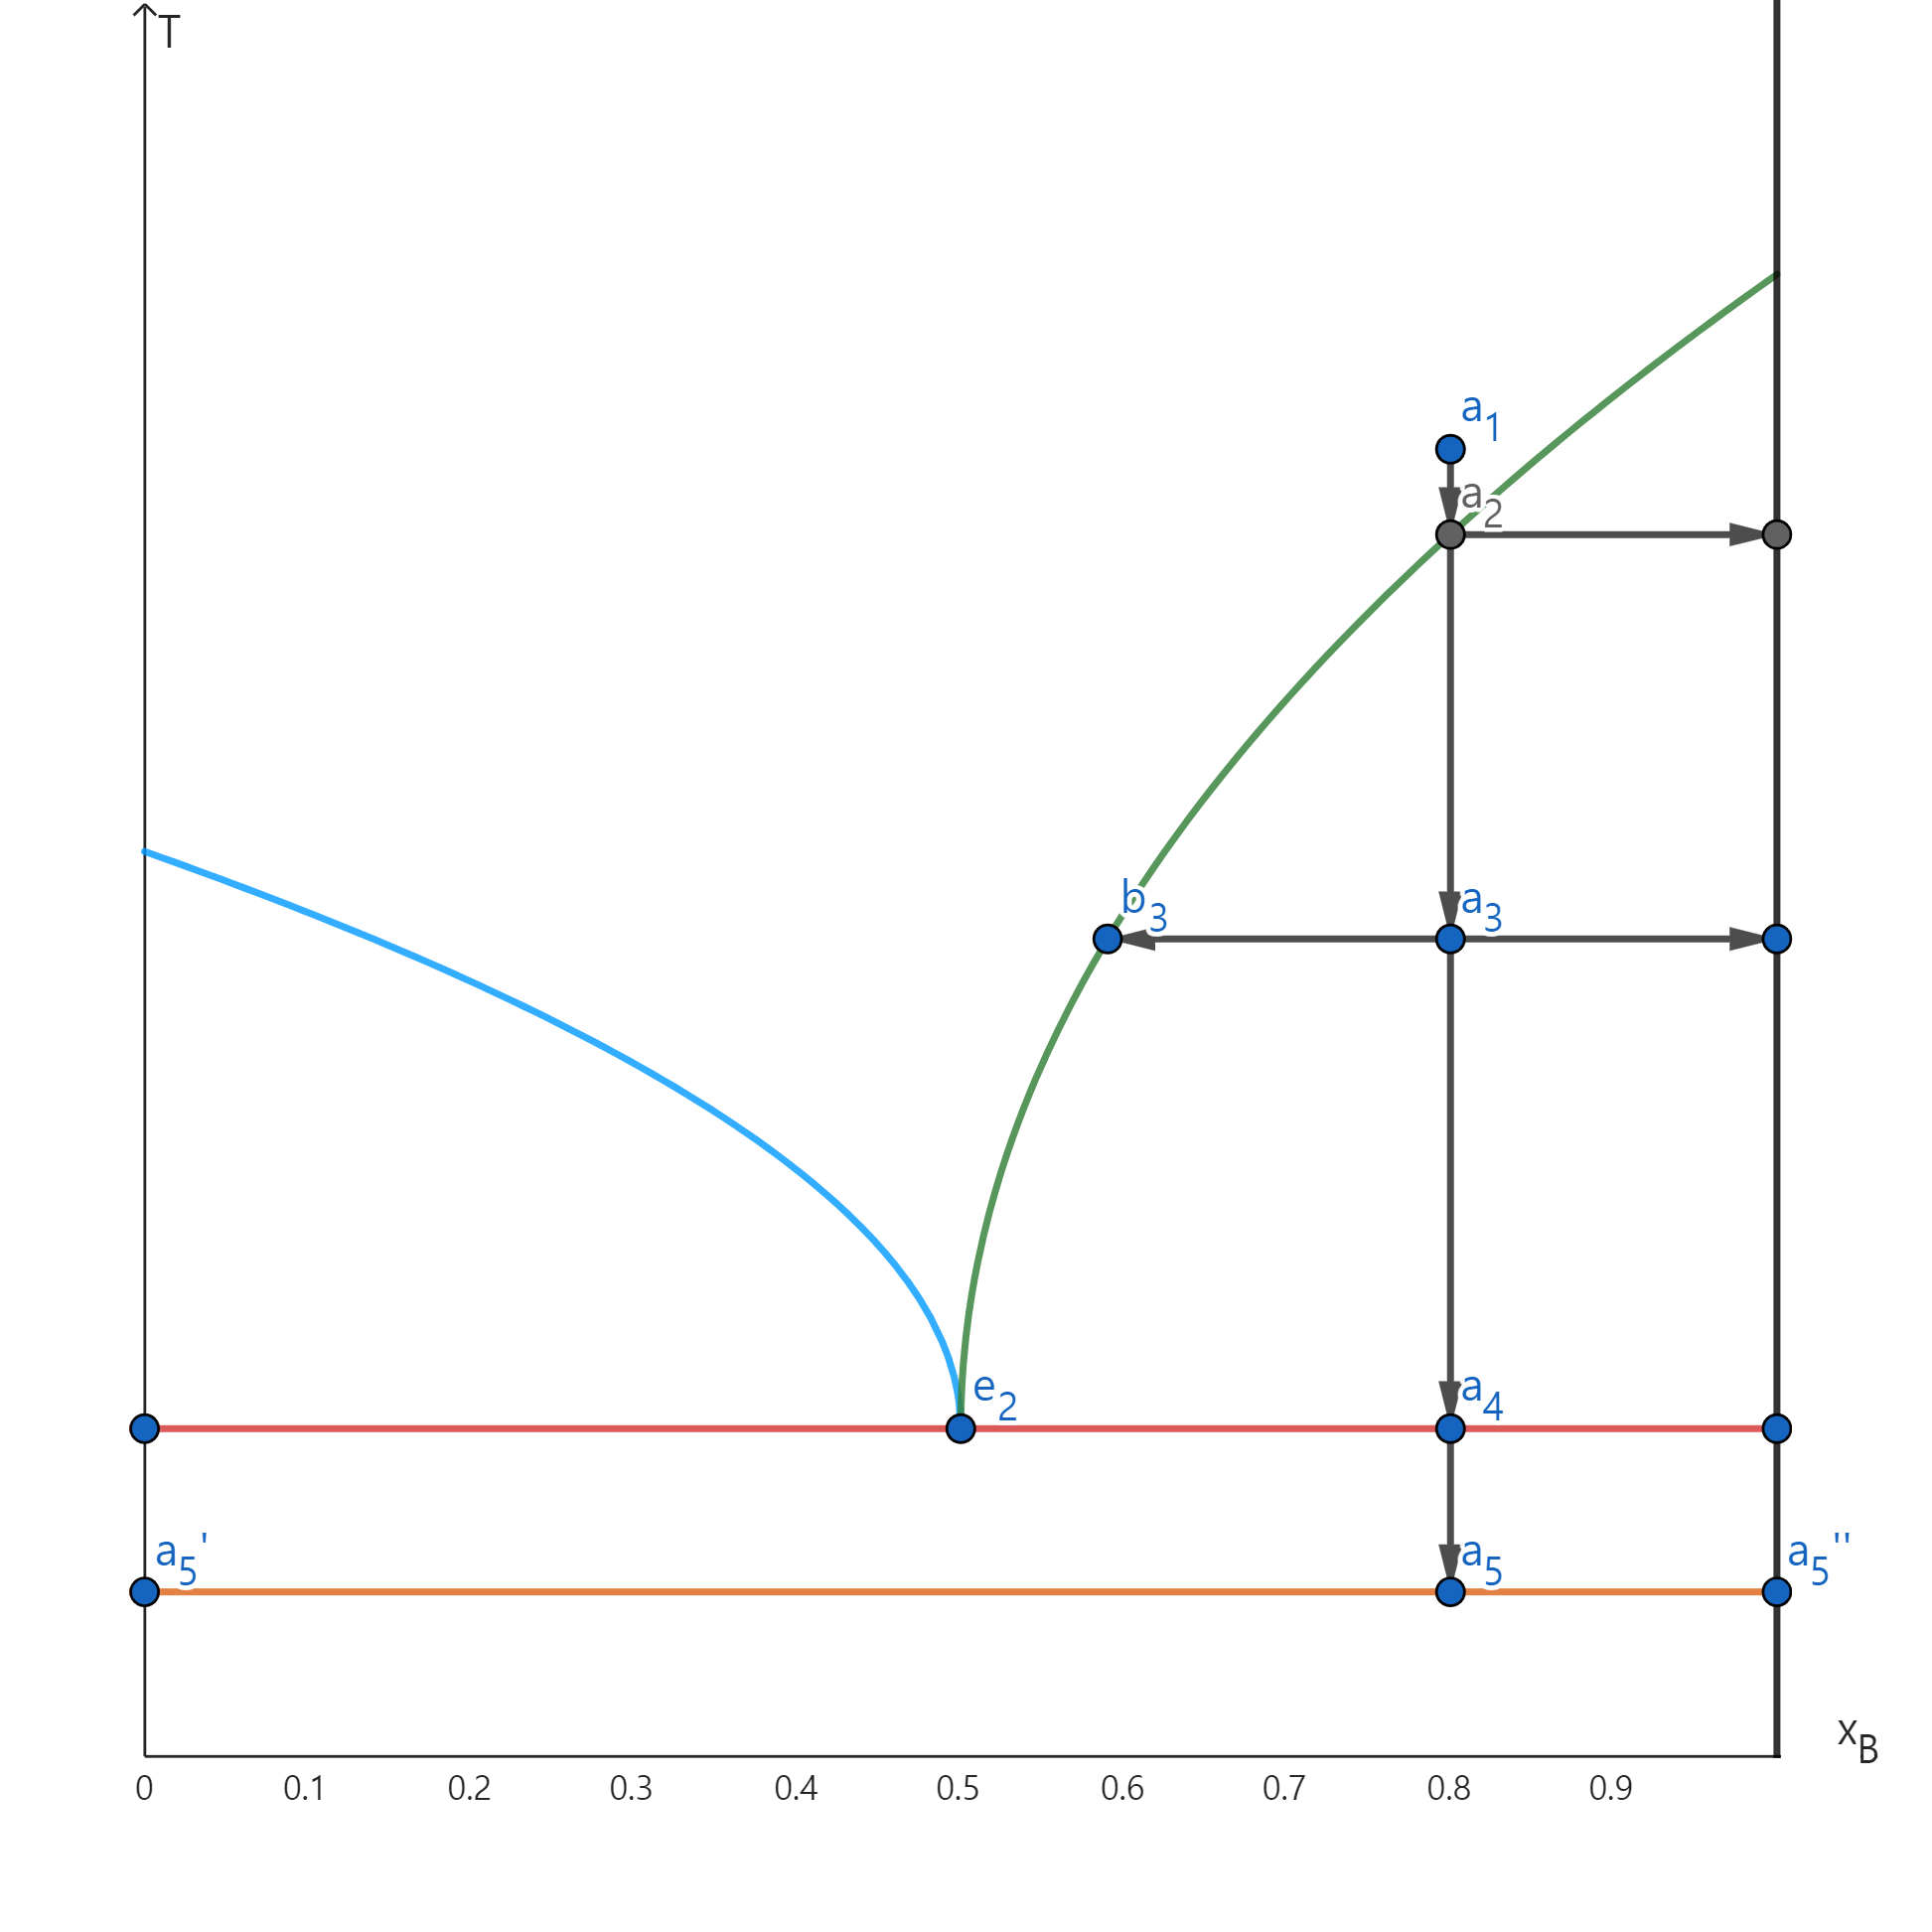
\includegraphics[width=0.7\linewidth]{Images/eutectic}
            \caption{고체-액체 상평형도}\label{f13}
        \end{figure}
        \par $a_1$에서 출발하자. $a_2$에 도달하면, B 고체가 생성되기 시작한다. $a_3$까지 온도를 내리면, 순수한 B 고체가 더 생성되고 $b_3$에 해당하는 액체가 남는다. 
        이제 $a_4$까지 내리자. 이제 액체의 분율은 $e_2$까지 내려간다. 이 이후로 온도가 더 내려가면 순수한 A 고체와 순수한 B 고체가 생성된다. 
        \par 이때 $e_2$ 점의 등치선은 \textbf{공정(Eutectic)}이라고 한다. 공정일 때 녹는점이 가장 낮고, 또한 이와 같은 분율일 때 액체를 냉각하면 순수한 A나 B가 만들어지지 
        않고 \textbf{판상(Lamellar)} 구조가 형성된다. 이러한 공정 상태를 알아내는 데에는 열 분석이 쓰일 수 있다. 특정 분율에서 등치선대로 온도를 내릴 때, 
        위의 Figure \ref{f13}에서 살펴보면 $a_1 \rightarrow a_2$에서 온도가 빠르게 하강하다가 $a_2 \rightarrow a_3$일 때 하강 속도가 느려지면서 순수한 B가 형성된다. 
        이후 $a_3 \rightarrow a_4$일 때 온도 변화가 없다. 이러한 온도 변화가 없는 지점을 \textbf{공정 중단(Eutectic halt)}이라고 한다.
        \par 다음과 같은, 화합물이 존재하는 상평형도(Figure \ref{f14})를 생각하자:\\
        \begin{figure}[H]
            \centering
            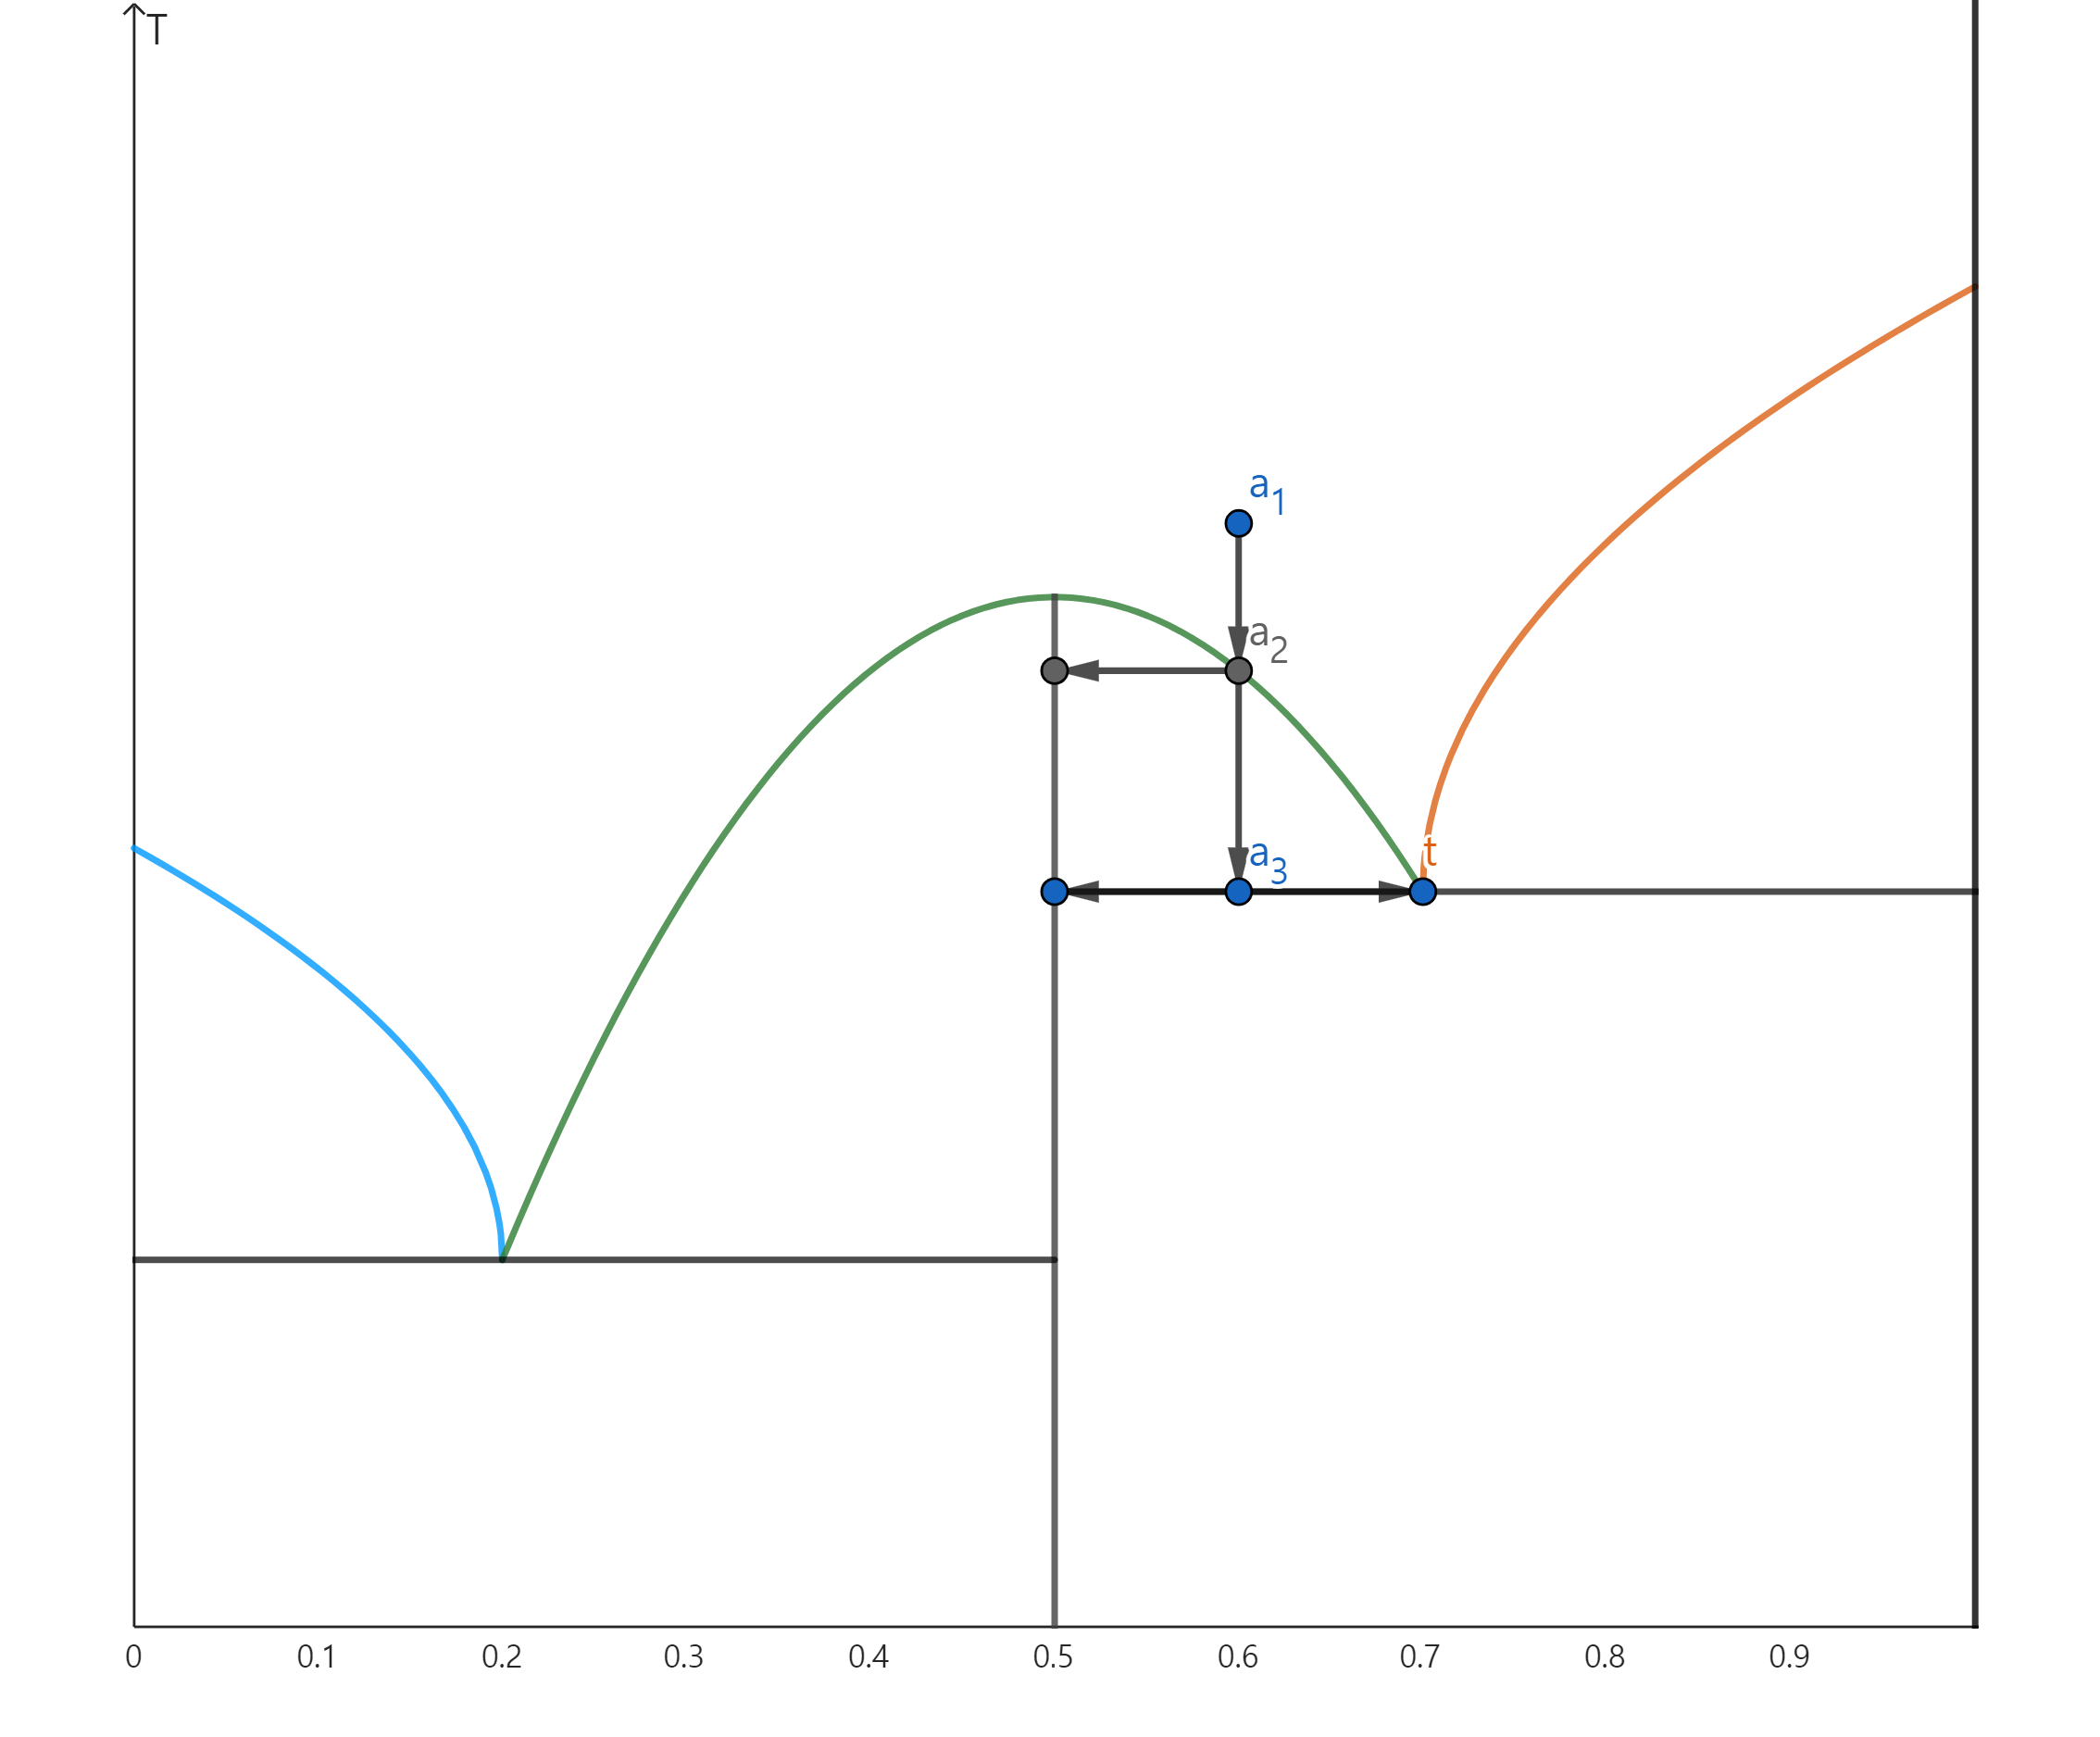
\includegraphics[scale=11]{Images/reactsys}
            \caption{화합물이 존재하는 고체-액체 상평형도}\label{f14}
        \end{figure}
        이 경우, 상평형도 여러 개로 쪼개어 생각할 수 있다. 즉, Figure \ref{f14}에서 왼쪽은 C, 오른쪽은 순수한 B가 존재하는 상평형도와, 왼쪽은 순수한 A, 오른쪽은 
        C가 존재하는 상평형도로 생각할 수 있다. (단, 가운데 화합물이 C라고 하자.) 이때 이 화합물 C는 이 분율을 유지하며 융해된다. 이를 \textbf{동질 용융(Congruent melting)}이라 
        한다. 그렇지 않은 경우를 \textbf{비동질 용융(Incongruent melting)}이라고 하는데, 이는 액체 화합물이 불안정하여 다른 상으로 분리되는 것을 의미한다.
    \section{삼원계 상평형도}
        \hspace{\parindent} 다음 Figure \ref{f15}와 같은 상평형도를 
        \textbf{삼원계 상평형도(Phase diagram of ternary system)}라 한다.
        \begin{figure}[H]
            \centering
            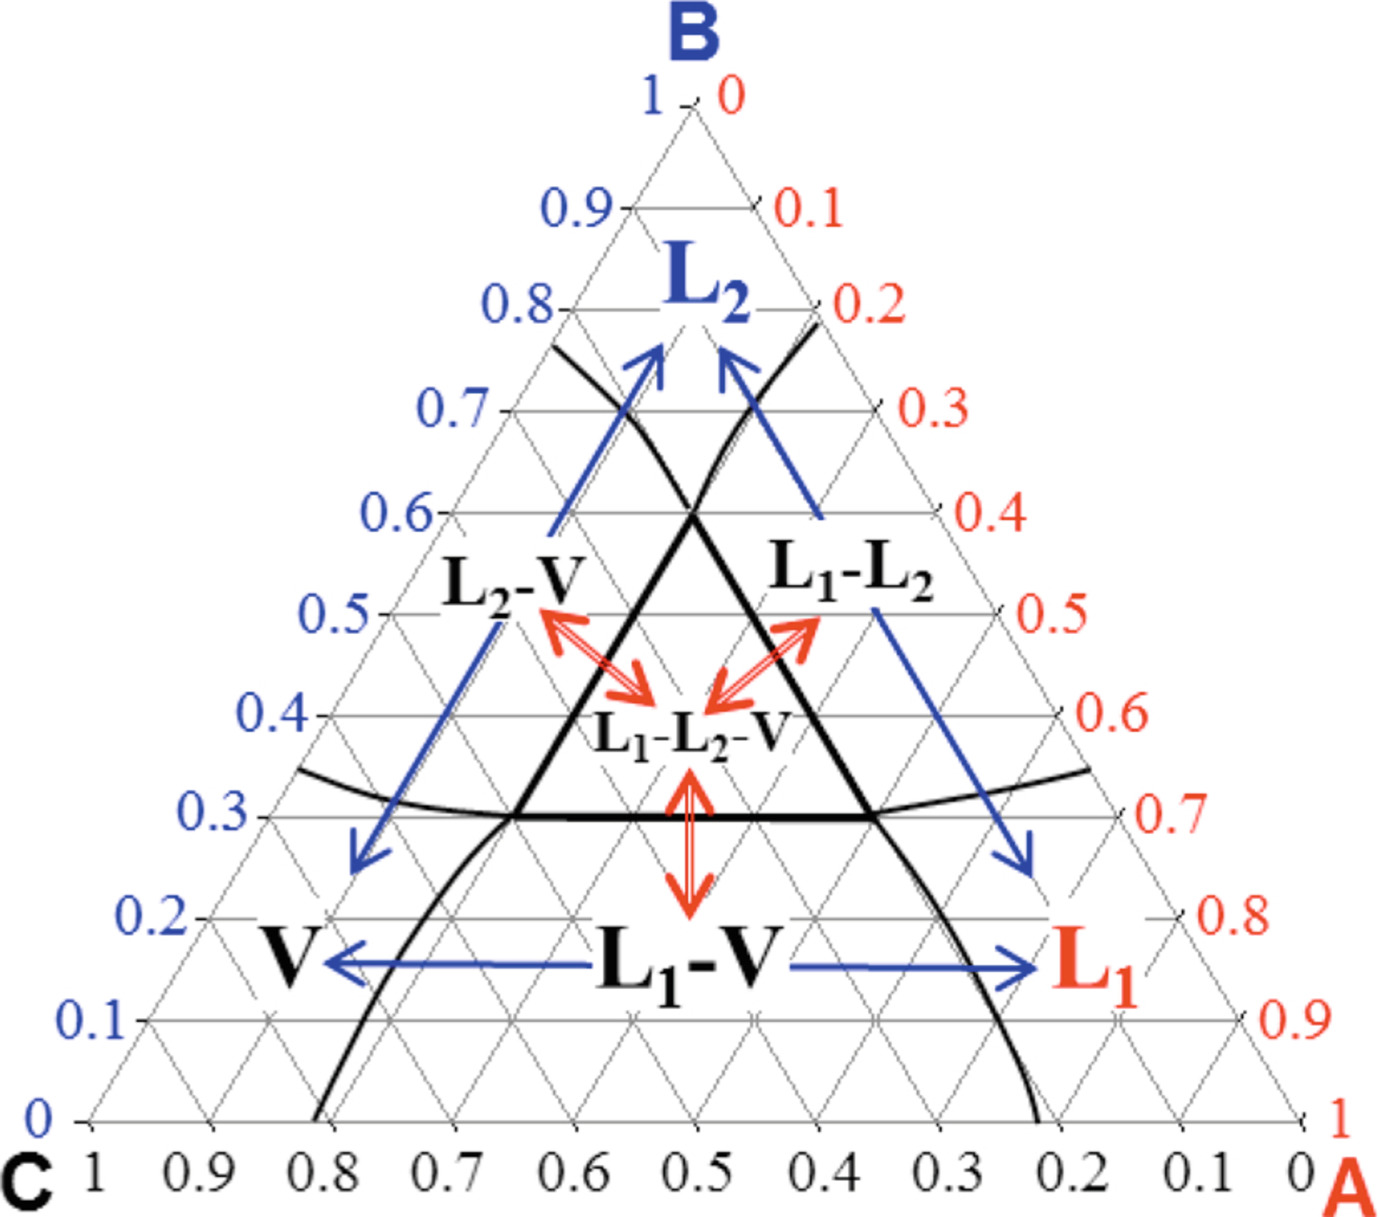
\includegraphics[width=0.6\textwidth]{Images/ternary}
            \caption{삼원계 상평형도}\label{f15}\cite{SMITH2013175}
        \end{figure}
        이때 밑변에서 1을 향하는 선에 수직인 선을 기준으로 성분의 분율을 읽어야 한다. 만약 삼원계 상평형도에서 서로 부분적으로 섞이는 쌍이 있을 경우, \ref{ch5sub3}에서의 논의를 마찬가지로 
        진행할 수 있다. 이러한 예시로는 물-아세트산-클로로폼의 혼합물로, 그 상평형도는 다음 Figure \ref{f16}과 같다. 
        \begin{figure}[H]
            \centering
            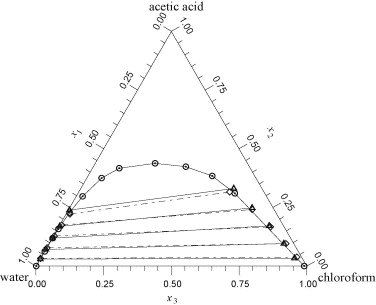
\includegraphics[width=0.6\textwidth]{Images/wtcternary}
            \caption{삼원계 상평형도}\label{f16}\cite{SENOL200651}
        \end{figure}
        이때 상이 분리되기 시작하는 지점을 \textbf{플레이트 포인트(Plait point)}라고 한다. 여기에서 상이 분리되는 두 점을 이은 선을 \textbf{대응선(Tie line)}이라 하고, 실험적으로 결정된다.
        고체에서도 마찬가지로 삼원계 상평형도를 결정할 수 있다.
    \section{활동도}
        \hspace{\parindent} 기체에서 화학 퍼텐셜은 $\mu_A = \mu_A^\ast + RT\ln{\left(p_A/p_A^\ast\right)}$와 같이 정의됨을 
        식 \ref{chempotgas}에서 살펴보았다. 이상 용액에서는 Raoult 법칙을 따르므로, $p_A = x_A p_A^\ast$가 성립한다는 사실에서 
        용액의 화학 퍼텐셜 $\mu_A = \mu_A^\ast +RT\ln{x_A}$가 성립한다. 실제 용액에서는 용질의 몰 분율 $x_A$ 대신 
        \textbf{활동도(Activity, $a_A$)}를 이용하여 다음과 같이 쓴다:
        \begin{equation*}
            \mu_A = \mu_A^\ast +RT\ln{a_A}
        \end{equation*}
        기체에서는 다음과 같이 정의된다:
        \begin{equation*}
            a_A = \frac{p_A}{p_A^\ast}
        \end{equation*}
        이러한 활동도는 '실효' 몰 분율로 볼 수 있다. 
        \par 모든 용매는 용질의 몰 분율이 0에 다가갈수록 Raoult 법칙을 따르므로, $a_A\rightarrow x_A$가 $x_A\rightarrow 1$일 때 성립한다. 
        이때 \textbf{활동도 계수(Activity coefficient, $\gamma_A$)}를 다음과 같이 정의한다:
        \begin{equation*}
            a_A = \gamma_A x_A
        \end{equation*}
        이때 $x_A\rightarrow 1$이면 $\gamma \rightarrow 1$이 모든 온도와 압력에서 성립한다. 따라서 화학 퍼텐셜은 다음과 같이 쓸 수 있다:
        \begin{equation*}
            \mu_A = \mu_A^\ast + RT\ln{x_A} + RT\ln{\gamma_A}
        \end{equation*}
        용매의 표준 상태는 $x_A=1$이고 압력이 $1$ bar일 때이다.
        \par Henry 법칙이 성립하는 이상 묽은 용액에서(즉, $x_B\rightarrow 0$), $p_B = K_B x_B$가 성립하므로 B의 화학 퍼텐셜은 
        \begin{equation*}
            \begin{aligned}
                \mu_B &= \mu_B^\ast +RT\ln{\frac{p_B}{p_B^\ast}} = \mu_B^\ast +RT \ln{\frac{K_B x_B}{p_B^\ast}}\\
                &= \mu_B^\ast +RT\ln{\frac{K_B}{p_B^\ast}}+RT\ln{x_B}
            \end{aligned}
        \end{equation*}
        이때 이상 묽은 용액에서 용질의 표준 화학 퍼텐셜을 다음과 같이 정의한다:
        \begin{defn}[이상 묽은 용액에서 용질의 표준 화학 퍼텐셜]
        \begin{equation*}
            \mu_B^\circlehbar = \mu_B^\ast +RT\ln{\frac{K_B}{p_B^\ast}}
        \end{equation*}
        \end{defn}
        따라서 이상 묽은 용액의 화학 퍼텐셜은 다음과 같이 다시 쓸 수 있다:
        \begin{equation*}
            \mu_B = \mu_B^\circlehbar + RT\ln{x_B}
        \end{equation*}
        만약 용액이 이상적이면, $K_B = p_B^\ast$이고 이는 Raoult 법칙에 해당한다. 따라서 이때 $\mu_B^\circlehbar = \mu_B^\ast$가 
        성립한다.
        \par 실제 용액에서는 다음과 같이 거동한다:
        \begin{equation*}
            \mu_B = \mu_B^\circlehbar + RT\ln{a_B}
        \end{equation*}
        이상 용액에서의 식과 실제 용액에서의 식을 각각 전개하여 합치면, 
        \begin{equation*}
            \begin{aligned}
                \mu_B &= \mu_B^\circlehbar - RT\ln{\frac{K_B}{p_B^\ast}} + RT \ln{\frac{p_B}{p_B^\ast}} \\
                &= \mu_B^\ast + RT\ln{\frac{p_B}{K_B}}
            \end{aligned}
        \end{equation*}
        과 같다. 따라서 활동도를 다음과 같이 정의할 수 있다:
        \begin{defn}[실제 용액에서의 용질의 활동도]
        \begin{equation*}
            a_B = \frac{p_B}{K_B}
        \end{equation*}
        \end{defn}
        마찬가지로 활동도 계수 또한 다음과 같이 정의된다:
        \begin{equation*}
            a_B = \gamma_B x_B
        \end{equation*}
        만약 $x_B \rightarrow 0$일 때 이상 묽은 용액의 거동을 따르므로, 이 경우 $a_B \rightarrow x_B$와 $\gamma_B \rightarrow 1$이 
        모든 온도와 압력에서 성립한다.
        \par 몰 분율 대신 몰랄 농도를 이용하여 다시 정의할 수 있다. 몰랄 농도를 $b$로 나타내면, 다음이 성립한다:
        \begin{equation*}
            \mu_B = \mu_B^\circlehbar +RT \ln{\frac{b_B}{b^\circlehbar}}
        \end{equation*}
        이때의 $\mu_B^\circlehbar$은 몰 분율을 이용할 때의 $\mu_B^\circlehbar$과 다른 값이다. 즉 $b = b^\circlehbar$일 때의 화학 퍼텐셜이다.
        이때 $b_B\rightarrow 0$일 때, $\mu_B \rightarrow -\infty$이다. 이는, 용액을 무한히 묽히면 용액이 무한히 안정해짐을 나타낸다. 
        실제 상황에 대입하면, 용액을 완벽히 분리하는 것이 매우 어려움을 나타낸다. 이때 실제 용액의 활동도 (계수)는 다음과 같이 정의한다:
        \begin{equation*}
            a_B = \gamma_B \frac{b_B}{b^\circlehbar}
        \end{equation*}
        이때 $b_B \rightarrow 0$일 때 $\gamma_B \rightarrow 1$이 성립한다. 따라서 실제 용액에서도 몰랄 농도를 이용해 다음과 같이 쓸 수 있다:
        \begin{equation*}
            \mu_B = \mu_B^\circlehbar + RT\ln{a_B}
        \end{equation*}
        \par 정규 용액에서는, 식 \ref{reggibbs}에서 출발한다. 이상 용액의 \\
        $$
        \Delta_\mathrm{mix}G = nRT\left\{x_A\ln{x_A} + x_B\ln{x_B}\right\}
        $$
        에서, 이상 용액이 아닐 경우에는 식이 다음과 같이 변화한다:
        \begin{equation*}
            \Delta_\mathrm{mix}G = nRT\left\{x_A\ln{a_A} + x_B\ln{a_B}\right\}
        \end{equation*}
        활동도 계수 표현으로 바꾸면 다음과 같다:
        \begin{equation*}
            \begin{aligned}
                \Delta_\mathrm{mix}G &= nRT\left\{x_A\ln{x_A\gamma_A}+x_B\ln{x_B\gamma_B}\right\}\\
                &= nRT\left\{x_A\ln{x_A} + x_B\ln{x_B}+x_A\ln{\gamma_A}+x_B\ln{\gamma_B}\right\}
            \end{aligned}
        \end{equation*}
        두 식을 합치기 위해 $\ln{\gamma_A} = \xi {x_B}^2$와 $\ln{\gamma_B} = \xi {x_A}^2$로 치환하면, 
        다음이 성립한다:
        \begin{obs}[Margules 등식]
        \begin{equation*}
            x_A \ln{\gamma_A}+x_B\ln{\gamma_B} = \xi x_A {x_B}^2+\xi x_B {x_A}^2 = \xi\left(x_A+x_B\right)x_A x_B = \xi x_A x_B
        \end{equation*}
        \end{obs}
        따라서 이렇게 활동도 계수를 $\xi$에 대해 나타낸 등식을 
        \textbf{Margules 등식(Margules equations)}이라 한다. 이를 이용하면 다음과 같이 쓸 수 있다:
        \begin{equation*}
            a_A = \gamma_A x_A = x_A e^{\xi {x_B}^2}=x_A e^{\xi \left(1-x_A\right)^2}
        \end{equation*}
        활동도의 정의로부터, 증기 압력에 대해 다음이 성립한다:
        \begin{equation*}
            p_A = p_A^\ast x_A e^{\xi\left(1-x_A\right)^2}
        \end{equation*}
        $\xi$의 부호에 따라 다음이 성립한다:
        \begin{enum}
            \item $\xi=0$이면, 이상 용액이므로 $p_A = p_A^\ast x_A$가 성립하고 따라서 Raoult 법칙이 성립한다.
            \item $\xi>0$이면, $\Delta_\mathrm{mix}H > 0$이고 용질-용매 간 상호작용이 선호되지 않으므로 이상 용액보다 증기 압력이 더 높다. 
            \item $\xi<0$이면, $\Delta_\mathrm{mix}H<0$이고 용질-용매 간 상호작용이 선호되므로 이상 용액보다 증기 압력이 더 낮다. 
        \end{enum}
        이상 용액에 가까워질 경우($x_A\rightarrow 1$), Raoult 법칙을 따라가게 되고 마찬가지로 $p_A = p_A^\ast x_A$를 만족한다. 
        $x_A <\!< 1$일 경우, 증기 압력은 다음으로 수렴한다:
        \begin{equation*}
            p_A = p_A^\ast x_A e^\xi
        \end{equation*}
        이를 통해 Henry 법칙에서 $K=e^\xi p_A^\ast$를 따라감을 알 수 있다.
        \par 이제 이온의 활동도를 정의하자. 몰랄 농도를 이온의 활동도로 이용하기 위해서는 용액이 매우 묽어야 한다(총 이온 농도로 $<1\textrm{ mmol kg}^{-1}$). 
        따라서 이온의 활동도를 따로 정의할 필요가 있다. 양이온의 화학 퍼텐셜을 $\mu_{+}$로, 음이온의 화학 퍼텐셜을 $\mu_{-}$로 쓰면, 
        전기적으로 중성인 용액의 몰 Gibbs 에너지는 이들의 합에 해당한다. 따라서 이상 용액에서는 다음이 성립한다:
        \begin{equation*}
            G_m^{\mathrm{ideal}}=\mu_{+}^\mathrm{ideal}+\mu_{-}^\mathrm{ideal}
        \end{equation*}
        또한 $\mu_J^\mathrm{ideal}=\mu_J^\circlehbar + RT\ln{x_J}$이다. 실제 용액에서는 다음과 같은 식을 이용해야 한다:
        \begin{equation*}
            \mu_J = \mu_J^\circlehbar + RT\ln{a_J}
        \end{equation*}
        이때 $a_J = x_J \gamma_J$이고, 따라서 $\mu_J = \mu_J^\mathrm{ideal}+RT\ln{\gamma_J}$이다. 따라서 실제 용액에서는 다음이 성립한다:
        \begin{equation*}
            \begin{aligned}
                G_m &= \mu_{+}+\mu_{-}=\mu_{+}^\mathrm{ideal}+\mu_{-}^\mathrm{ideal}+RT\ln{\gamma_{+}}+RT\ln{\gamma_{-}}\\
                &= G_m^\mathrm{ideal}+RT\ln{\gamma_{+} \gamma_{-}}
            \end{aligned}
        \end{equation*}
        이때 마지막 항이 이상 용액으로부터의 편차를 나타낸다.
        \par 그러나, 실험적으로 $\gamma_{+}$와 $\gamma_{-}$를 각각 구할 방법은 존재하지 않는다. 따라서 이들의 기하평균으로 
        \textbf{평균 활동도 계수(Mean activity coefficient, $\gamma_{\pm}$)}를 정의한다. 즉, q가 양이온과 p가 음이온(즉 $M_p X_q$)이 
        있을 때, 평균 활동도 계수는 다음과 같이 정의된다:
        \begin{defn}[평균 활동도 계수]
        \begin{equation*}
            \gamma_\pm = \left({\gamma_{+}}^p{\gamma_{-}}^q\right)^{1/s},\, s=p+q
        \end{equation*}
        \end{defn}
        따라서 각 이온의 화학 퍼텐셜은 다음과 같이 쓸 수 있다:
        \begin{equation*}
            \mu_i = \mu_i^\mathrm{ideal}+RT\ln{\gamma_\pm}
        \end{equation*}
        \par 이상 용액으로부터 실제 용액이 가지는 편차는 \textbf{Debye-Hückel 한계 법칙(Debye-Hückel limiting law)}로 설명한다. 
        먼저, 이온 주변에 반대 전하의 이온이 위치할 가능성이 크다는 것을 가정한다. 이러한 이온 주변의 영역을 \textbf{이온 분위기(Ionic atmosphere)}라 한다. 
        이를 통해 중심 이온의 화학 퍼텐셜은 낮아진다. 이 차이가 이상 용액과 실제 용액의 몰 Gibbs 에너지 차이를 만들어낸다. 다음과 같은 
        식을 \textbf{Debye-Hückel 한계 법칙}이라 한다:
        \begin{law}[Debye-Hückel 한계 법칙]
        \begin{equation*}
            \log{\gamma_\pm}=-A\left\vert z_{+}z_{-}\right\vert I^{1/2}
        \end{equation*}
        \end{law}
        이때 25 $^\circ C$의 수용액에서 $A = 0.509$이고, $I$는 \textbf{이온 세기(Ionic strength)}라 하며 다음과 같이 정의한다:
        \begin{defn}[이온 세기]
        \begin{equation*}
            I = \frac{1}{2}\sum_{i}{z_i}^2\left(b_i/b^\circlehbar\right)
        \end{equation*}
        \end{defn}
        여기에서 $z_i$는 이온의 가수, $b_i$는 이온의 몰랄 농도이다. 만약 두 종류의 이온만 존재한다면 이온 세기는 다음과 같이 정의된다:
        \begin{equation*}
            I = \frac{1}{2}\frac{b_{+}{z_{+}}^2+b_{-}{z_{-}}^2}{b^\circlehbar}
        \end{equation*}
        \par 이러한 Debye-Hückel 한계 법칙은 낮은 농도에서는 잘 맞으나, 높은 농도에서는 오차가 발생한다. 이와 같은 
        한계를 보완하기 위해 \textbf{확장된 Debye-Hückel 법칙(Extended Debye-Hückel law, 또는 Truesdell-Jones 등식으로도 불림)}을 도입한다:
        \begin{law}[확장된 Debye-Hückel 법칙]
        \begin{equation*}
            \log{\gamma_\pm}=-\frac{A \left\vert z_{+}z_{-}\right\vert I^{1/2}}{1+BI^{1/2}}
        \end{equation*}
        \end{law}
        여기에서 $B$는 단위 없는 상수이다. 더 확장하면 다음과 같은 \textbf{Davies 등식(Davies equation)}을 얻을 수 있다:
        \begin{law}[Davies 등식]
        \begin{equation*}
            \log{\gamma_\pm}=-\frac{A \left\vert z_{+}z_{-}\right\vert I^{1/2}}{1+BI^{1/2}}+CI
        \end{equation*}
        \end{law}
        다만 Davies 등식을 이용하여도 0.1 mol kg$^{-1}$ 정도까지만 잘 맞는다. 따라서 여러 모형과 Gibbs-Duhem 등식(\ref{gibbsduhem} 참고)을 
        이용하여 용질의 활동도 계수를 추측한다. 
        \par 기체에서는 \textbf{퓨가시티(Fugacity, $f$)}를 정의한다. 퓨가시티는 다음과 같이 정의한다:
        \begin{defn}[퓨가시티]
        \begin{equation*}
            f=\gamma p
        \end{equation*}
        \end{defn}
        퓨가시티는 기체의 활동도로 볼 수 있다.